\documentclass[11pt]{article}

    \usepackage[breakable]{tcolorbox}
    \usepackage{parskip} % Stop auto-indenting (to mimic markdown behaviour)
    
    \usepackage{iftex}
    \ifPDFTeX
    	\usepackage[T1]{fontenc}
    	\usepackage{mathpazo}
    \else
    	\usepackage{fontspec}
    \fi

    % Basic figure setup, for now with no caption control since it's done
    % automatically by Pandoc (which extracts ![](path) syntax from Markdown).
    \usepackage{graphicx}
    % Maintain compatibility with old templates. Remove in nbconvert 6.0
    \let\Oldincludegraphics\includegraphics
    % Ensure that by default, figures have no caption (until we provide a
    % proper Figure object with a Caption API and a way to capture that
    % in the conversion process - todo).
    \usepackage{caption}
    \DeclareCaptionFormat{nocaption}{}
    \captionsetup{format=nocaption,aboveskip=0pt,belowskip=0pt}

    \usepackage{float}
    \floatplacement{figure}{H} % forces figures to be placed at the correct location
    \usepackage{xcolor} % Allow colors to be defined
    \usepackage{enumerate} % Needed for markdown enumerations to work
    \usepackage{geometry} % Used to adjust the document margins
    \usepackage{amsmath} % Equations
    \usepackage{amssymb} % Equations
    \usepackage{textcomp} % defines textquotesingle
    % Hack from http://tex.stackexchange.com/a/47451/13684:
    \AtBeginDocument{%
        \def\PYZsq{\textquotesingle}% Upright quotes in Pygmentized code
    }
    \usepackage{upquote} % Upright quotes for verbatim code
    \usepackage{eurosym} % defines \euro
    \usepackage[mathletters]{ucs} % Extended unicode (utf-8) support
    \usepackage{fancyvrb} % verbatim replacement that allows latex
    \usepackage{grffile} % extends the file name processing of package graphics 
                         % to support a larger range
    \makeatletter % fix for old versions of grffile with XeLaTeX
    \@ifpackagelater{grffile}{2019/11/01}
    {
      % Do nothing on new versions
    }
    {
      \def\Gread@@xetex#1{%
        \IfFileExists{"\Gin@base".bb}%
        {\Gread@eps{\Gin@base.bb}}%
        {\Gread@@xetex@aux#1}%
      }
    }
    \makeatother
    \usepackage[Export]{adjustbox} % Used to constrain images to a maximum size
    \adjustboxset{max size={0.9\linewidth}{0.9\paperheight}}

    % The hyperref package gives us a pdf with properly built
    % internal navigation ('pdf bookmarks' for the table of contents,
    % internal cross-reference links, web links for URLs, etc.)
    \usepackage{hyperref}
    % The default LaTeX title has an obnoxious amount of whitespace. By default,
    % titling removes some of it. It also provides customization options.
    \usepackage{titling}
    \usepackage{longtable} % longtable support required by pandoc >1.10
    \usepackage{booktabs}  % table support for pandoc > 1.12.2
    \usepackage[inline]{enumitem} % IRkernel/repr support (it uses the enumerate* environment)
    \usepackage[normalem]{ulem} % ulem is needed to support strikethroughs (\sout)
                                % normalem makes italics be italics, not underlines
    \usepackage{mathrsfs}
    

    
    % Colors for the hyperref package
    \definecolor{urlcolor}{rgb}{0,.145,.698}
    \definecolor{linkcolor}{rgb}{.71,0.21,0.01}
    \definecolor{citecolor}{rgb}{.12,.54,.11}

    % ANSI colors
    \definecolor{ansi-black}{HTML}{3E424D}
    \definecolor{ansi-black-intense}{HTML}{282C36}
    \definecolor{ansi-red}{HTML}{E75C58}
    \definecolor{ansi-red-intense}{HTML}{B22B31}
    \definecolor{ansi-green}{HTML}{00A250}
    \definecolor{ansi-green-intense}{HTML}{007427}
    \definecolor{ansi-yellow}{HTML}{DDB62B}
    \definecolor{ansi-yellow-intense}{HTML}{B27D12}
    \definecolor{ansi-blue}{HTML}{208FFB}
    \definecolor{ansi-blue-intense}{HTML}{0065CA}
    \definecolor{ansi-magenta}{HTML}{D160C4}
    \definecolor{ansi-magenta-intense}{HTML}{A03196}
    \definecolor{ansi-cyan}{HTML}{60C6C8}
    \definecolor{ansi-cyan-intense}{HTML}{258F8F}
    \definecolor{ansi-white}{HTML}{C5C1B4}
    \definecolor{ansi-white-intense}{HTML}{A1A6B2}
    \definecolor{ansi-default-inverse-fg}{HTML}{FFFFFF}
    \definecolor{ansi-default-inverse-bg}{HTML}{000000}

    % common color for the border for error outputs.
    \definecolor{outerrorbackground}{HTML}{FFDFDF}

    % commands and environments needed by pandoc snippets
    % extracted from the output of `pandoc -s`
    \providecommand{\tightlist}{%
      \setlength{\itemsep}{0pt}\setlength{\parskip}{0pt}}
    \DefineVerbatimEnvironment{Highlighting}{Verbatim}{commandchars=\\\{\}}
    % Add ',fontsize=\small' for more characters per line
    \newenvironment{Shaded}{}{}
    \newcommand{\KeywordTok}[1]{\textcolor[rgb]{0.00,0.44,0.13}{\textbf{{#1}}}}
    \newcommand{\DataTypeTok}[1]{\textcolor[rgb]{0.56,0.13,0.00}{{#1}}}
    \newcommand{\DecValTok}[1]{\textcolor[rgb]{0.25,0.63,0.44}{{#1}}}
    \newcommand{\BaseNTok}[1]{\textcolor[rgb]{0.25,0.63,0.44}{{#1}}}
    \newcommand{\FloatTok}[1]{\textcolor[rgb]{0.25,0.63,0.44}{{#1}}}
    \newcommand{\CharTok}[1]{\textcolor[rgb]{0.25,0.44,0.63}{{#1}}}
    \newcommand{\StringTok}[1]{\textcolor[rgb]{0.25,0.44,0.63}{{#1}}}
    \newcommand{\CommentTok}[1]{\textcolor[rgb]{0.38,0.63,0.69}{\textit{{#1}}}}
    \newcommand{\OtherTok}[1]{\textcolor[rgb]{0.00,0.44,0.13}{{#1}}}
    \newcommand{\AlertTok}[1]{\textcolor[rgb]{1.00,0.00,0.00}{\textbf{{#1}}}}
    \newcommand{\FunctionTok}[1]{\textcolor[rgb]{0.02,0.16,0.49}{{#1}}}
    \newcommand{\RegionMarkerTok}[1]{{#1}}
    \newcommand{\ErrorTok}[1]{\textcolor[rgb]{1.00,0.00,0.00}{\textbf{{#1}}}}
    \newcommand{\NormalTok}[1]{{#1}}
    
    % Additional commands for more recent versions of Pandoc
    \newcommand{\ConstantTok}[1]{\textcolor[rgb]{0.53,0.00,0.00}{{#1}}}
    \newcommand{\SpecialCharTok}[1]{\textcolor[rgb]{0.25,0.44,0.63}{{#1}}}
    \newcommand{\VerbatimStringTok}[1]{\textcolor[rgb]{0.25,0.44,0.63}{{#1}}}
    \newcommand{\SpecialStringTok}[1]{\textcolor[rgb]{0.73,0.40,0.53}{{#1}}}
    \newcommand{\ImportTok}[1]{{#1}}
    \newcommand{\DocumentationTok}[1]{\textcolor[rgb]{0.73,0.13,0.13}{\textit{{#1}}}}
    \newcommand{\AnnotationTok}[1]{\textcolor[rgb]{0.38,0.63,0.69}{\textbf{\textit{{#1}}}}}
    \newcommand{\CommentVarTok}[1]{\textcolor[rgb]{0.38,0.63,0.69}{\textbf{\textit{{#1}}}}}
    \newcommand{\VariableTok}[1]{\textcolor[rgb]{0.10,0.09,0.49}{{#1}}}
    \newcommand{\ControlFlowTok}[1]{\textcolor[rgb]{0.00,0.44,0.13}{\textbf{{#1}}}}
    \newcommand{\OperatorTok}[1]{\textcolor[rgb]{0.40,0.40,0.40}{{#1}}}
    \newcommand{\BuiltInTok}[1]{{#1}}
    \newcommand{\ExtensionTok}[1]{{#1}}
    \newcommand{\PreprocessorTok}[1]{\textcolor[rgb]{0.74,0.48,0.00}{{#1}}}
    \newcommand{\AttributeTok}[1]{\textcolor[rgb]{0.49,0.56,0.16}{{#1}}}
    \newcommand{\InformationTok}[1]{\textcolor[rgb]{0.38,0.63,0.69}{\textbf{\textit{{#1}}}}}
    \newcommand{\WarningTok}[1]{\textcolor[rgb]{0.38,0.63,0.69}{\textbf{\textit{{#1}}}}}
    
    
    % Define a nice break command that doesn't care if a line doesn't already
    % exist.
    \def\br{\hspace*{\fill} \\* }
    % Math Jax compatibility definitions
    \def\gt{>}
    \def\lt{<}
    \let\Oldtex\TeX
    \let\Oldlatex\LaTeX
    \renewcommand{\TeX}{\textrm{\Oldtex}}
    \renewcommand{\LaTeX}{\textrm{\Oldlatex}}
    % Document parameters
    % Document title
    \title{Strings}
    
    
    
    
    
% Pygments definitions
\makeatletter
\def\PY@reset{\let\PY@it=\relax \let\PY@bf=\relax%
    \let\PY@ul=\relax \let\PY@tc=\relax%
    \let\PY@bc=\relax \let\PY@ff=\relax}
\def\PY@tok#1{\csname PY@tok@#1\endcsname}
\def\PY@toks#1+{\ifx\relax#1\empty\else%
    \PY@tok{#1}\expandafter\PY@toks\fi}
\def\PY@do#1{\PY@bc{\PY@tc{\PY@ul{%
    \PY@it{\PY@bf{\PY@ff{#1}}}}}}}
\def\PY#1#2{\PY@reset\PY@toks#1+\relax+\PY@do{#2}}

\@namedef{PY@tok@w}{\def\PY@tc##1{\textcolor[rgb]{0.73,0.73,0.73}{##1}}}
\@namedef{PY@tok@c}{\let\PY@it=\textit\def\PY@tc##1{\textcolor[rgb]{0.25,0.50,0.50}{##1}}}
\@namedef{PY@tok@cp}{\def\PY@tc##1{\textcolor[rgb]{0.74,0.48,0.00}{##1}}}
\@namedef{PY@tok@k}{\let\PY@bf=\textbf\def\PY@tc##1{\textcolor[rgb]{0.00,0.50,0.00}{##1}}}
\@namedef{PY@tok@kp}{\def\PY@tc##1{\textcolor[rgb]{0.00,0.50,0.00}{##1}}}
\@namedef{PY@tok@kt}{\def\PY@tc##1{\textcolor[rgb]{0.69,0.00,0.25}{##1}}}
\@namedef{PY@tok@o}{\def\PY@tc##1{\textcolor[rgb]{0.40,0.40,0.40}{##1}}}
\@namedef{PY@tok@ow}{\let\PY@bf=\textbf\def\PY@tc##1{\textcolor[rgb]{0.67,0.13,1.00}{##1}}}
\@namedef{PY@tok@nb}{\def\PY@tc##1{\textcolor[rgb]{0.00,0.50,0.00}{##1}}}
\@namedef{PY@tok@nf}{\def\PY@tc##1{\textcolor[rgb]{0.00,0.00,1.00}{##1}}}
\@namedef{PY@tok@nc}{\let\PY@bf=\textbf\def\PY@tc##1{\textcolor[rgb]{0.00,0.00,1.00}{##1}}}
\@namedef{PY@tok@nn}{\let\PY@bf=\textbf\def\PY@tc##1{\textcolor[rgb]{0.00,0.00,1.00}{##1}}}
\@namedef{PY@tok@ne}{\let\PY@bf=\textbf\def\PY@tc##1{\textcolor[rgb]{0.82,0.25,0.23}{##1}}}
\@namedef{PY@tok@nv}{\def\PY@tc##1{\textcolor[rgb]{0.10,0.09,0.49}{##1}}}
\@namedef{PY@tok@no}{\def\PY@tc##1{\textcolor[rgb]{0.53,0.00,0.00}{##1}}}
\@namedef{PY@tok@nl}{\def\PY@tc##1{\textcolor[rgb]{0.63,0.63,0.00}{##1}}}
\@namedef{PY@tok@ni}{\let\PY@bf=\textbf\def\PY@tc##1{\textcolor[rgb]{0.60,0.60,0.60}{##1}}}
\@namedef{PY@tok@na}{\def\PY@tc##1{\textcolor[rgb]{0.49,0.56,0.16}{##1}}}
\@namedef{PY@tok@nt}{\let\PY@bf=\textbf\def\PY@tc##1{\textcolor[rgb]{0.00,0.50,0.00}{##1}}}
\@namedef{PY@tok@nd}{\def\PY@tc##1{\textcolor[rgb]{0.67,0.13,1.00}{##1}}}
\@namedef{PY@tok@s}{\def\PY@tc##1{\textcolor[rgb]{0.73,0.13,0.13}{##1}}}
\@namedef{PY@tok@sd}{\let\PY@it=\textit\def\PY@tc##1{\textcolor[rgb]{0.73,0.13,0.13}{##1}}}
\@namedef{PY@tok@si}{\let\PY@bf=\textbf\def\PY@tc##1{\textcolor[rgb]{0.73,0.40,0.53}{##1}}}
\@namedef{PY@tok@se}{\let\PY@bf=\textbf\def\PY@tc##1{\textcolor[rgb]{0.73,0.40,0.13}{##1}}}
\@namedef{PY@tok@sr}{\def\PY@tc##1{\textcolor[rgb]{0.73,0.40,0.53}{##1}}}
\@namedef{PY@tok@ss}{\def\PY@tc##1{\textcolor[rgb]{0.10,0.09,0.49}{##1}}}
\@namedef{PY@tok@sx}{\def\PY@tc##1{\textcolor[rgb]{0.00,0.50,0.00}{##1}}}
\@namedef{PY@tok@m}{\def\PY@tc##1{\textcolor[rgb]{0.40,0.40,0.40}{##1}}}
\@namedef{PY@tok@gh}{\let\PY@bf=\textbf\def\PY@tc##1{\textcolor[rgb]{0.00,0.00,0.50}{##1}}}
\@namedef{PY@tok@gu}{\let\PY@bf=\textbf\def\PY@tc##1{\textcolor[rgb]{0.50,0.00,0.50}{##1}}}
\@namedef{PY@tok@gd}{\def\PY@tc##1{\textcolor[rgb]{0.63,0.00,0.00}{##1}}}
\@namedef{PY@tok@gi}{\def\PY@tc##1{\textcolor[rgb]{0.00,0.63,0.00}{##1}}}
\@namedef{PY@tok@gr}{\def\PY@tc##1{\textcolor[rgb]{1.00,0.00,0.00}{##1}}}
\@namedef{PY@tok@ge}{\let\PY@it=\textit}
\@namedef{PY@tok@gs}{\let\PY@bf=\textbf}
\@namedef{PY@tok@gp}{\let\PY@bf=\textbf\def\PY@tc##1{\textcolor[rgb]{0.00,0.00,0.50}{##1}}}
\@namedef{PY@tok@go}{\def\PY@tc##1{\textcolor[rgb]{0.53,0.53,0.53}{##1}}}
\@namedef{PY@tok@gt}{\def\PY@tc##1{\textcolor[rgb]{0.00,0.27,0.87}{##1}}}
\@namedef{PY@tok@err}{\def\PY@bc##1{{\setlength{\fboxsep}{\string -\fboxrule}\fcolorbox[rgb]{1.00,0.00,0.00}{1,1,1}{\strut ##1}}}}
\@namedef{PY@tok@kc}{\let\PY@bf=\textbf\def\PY@tc##1{\textcolor[rgb]{0.00,0.50,0.00}{##1}}}
\@namedef{PY@tok@kd}{\let\PY@bf=\textbf\def\PY@tc##1{\textcolor[rgb]{0.00,0.50,0.00}{##1}}}
\@namedef{PY@tok@kn}{\let\PY@bf=\textbf\def\PY@tc##1{\textcolor[rgb]{0.00,0.50,0.00}{##1}}}
\@namedef{PY@tok@kr}{\let\PY@bf=\textbf\def\PY@tc##1{\textcolor[rgb]{0.00,0.50,0.00}{##1}}}
\@namedef{PY@tok@bp}{\def\PY@tc##1{\textcolor[rgb]{0.00,0.50,0.00}{##1}}}
\@namedef{PY@tok@fm}{\def\PY@tc##1{\textcolor[rgb]{0.00,0.00,1.00}{##1}}}
\@namedef{PY@tok@vc}{\def\PY@tc##1{\textcolor[rgb]{0.10,0.09,0.49}{##1}}}
\@namedef{PY@tok@vg}{\def\PY@tc##1{\textcolor[rgb]{0.10,0.09,0.49}{##1}}}
\@namedef{PY@tok@vi}{\def\PY@tc##1{\textcolor[rgb]{0.10,0.09,0.49}{##1}}}
\@namedef{PY@tok@vm}{\def\PY@tc##1{\textcolor[rgb]{0.10,0.09,0.49}{##1}}}
\@namedef{PY@tok@sa}{\def\PY@tc##1{\textcolor[rgb]{0.73,0.13,0.13}{##1}}}
\@namedef{PY@tok@sb}{\def\PY@tc##1{\textcolor[rgb]{0.73,0.13,0.13}{##1}}}
\@namedef{PY@tok@sc}{\def\PY@tc##1{\textcolor[rgb]{0.73,0.13,0.13}{##1}}}
\@namedef{PY@tok@dl}{\def\PY@tc##1{\textcolor[rgb]{0.73,0.13,0.13}{##1}}}
\@namedef{PY@tok@s2}{\def\PY@tc##1{\textcolor[rgb]{0.73,0.13,0.13}{##1}}}
\@namedef{PY@tok@sh}{\def\PY@tc##1{\textcolor[rgb]{0.73,0.13,0.13}{##1}}}
\@namedef{PY@tok@s1}{\def\PY@tc##1{\textcolor[rgb]{0.73,0.13,0.13}{##1}}}
\@namedef{PY@tok@mb}{\def\PY@tc##1{\textcolor[rgb]{0.40,0.40,0.40}{##1}}}
\@namedef{PY@tok@mf}{\def\PY@tc##1{\textcolor[rgb]{0.40,0.40,0.40}{##1}}}
\@namedef{PY@tok@mh}{\def\PY@tc##1{\textcolor[rgb]{0.40,0.40,0.40}{##1}}}
\@namedef{PY@tok@mi}{\def\PY@tc##1{\textcolor[rgb]{0.40,0.40,0.40}{##1}}}
\@namedef{PY@tok@il}{\def\PY@tc##1{\textcolor[rgb]{0.40,0.40,0.40}{##1}}}
\@namedef{PY@tok@mo}{\def\PY@tc##1{\textcolor[rgb]{0.40,0.40,0.40}{##1}}}
\@namedef{PY@tok@ch}{\let\PY@it=\textit\def\PY@tc##1{\textcolor[rgb]{0.25,0.50,0.50}{##1}}}
\@namedef{PY@tok@cm}{\let\PY@it=\textit\def\PY@tc##1{\textcolor[rgb]{0.25,0.50,0.50}{##1}}}
\@namedef{PY@tok@cpf}{\let\PY@it=\textit\def\PY@tc##1{\textcolor[rgb]{0.25,0.50,0.50}{##1}}}
\@namedef{PY@tok@c1}{\let\PY@it=\textit\def\PY@tc##1{\textcolor[rgb]{0.25,0.50,0.50}{##1}}}
\@namedef{PY@tok@cs}{\let\PY@it=\textit\def\PY@tc##1{\textcolor[rgb]{0.25,0.50,0.50}{##1}}}

\def\PYZbs{\char`\\}
\def\PYZus{\char`\_}
\def\PYZob{\char`\{}
\def\PYZcb{\char`\}}
\def\PYZca{\char`\^}
\def\PYZam{\char`\&}
\def\PYZlt{\char`\<}
\def\PYZgt{\char`\>}
\def\PYZsh{\char`\#}
\def\PYZpc{\char`\%}
\def\PYZdl{\char`\$}
\def\PYZhy{\char`\-}
\def\PYZsq{\char`\'}
\def\PYZdq{\char`\"}
\def\PYZti{\char`\~}
% for compatibility with earlier versions
\def\PYZat{@}
\def\PYZlb{[}
\def\PYZrb{]}
\makeatother


    % For linebreaks inside Verbatim environment from package fancyvrb. 
    \makeatletter
        \newbox\Wrappedcontinuationbox 
        \newbox\Wrappedvisiblespacebox 
        \newcommand*\Wrappedvisiblespace {\textcolor{red}{\textvisiblespace}} 
        \newcommand*\Wrappedcontinuationsymbol {\textcolor{red}{\llap{\tiny$\m@th\hookrightarrow$}}} 
        \newcommand*\Wrappedcontinuationindent {3ex } 
        \newcommand*\Wrappedafterbreak {\kern\Wrappedcontinuationindent\copy\Wrappedcontinuationbox} 
        % Take advantage of the already applied Pygments mark-up to insert 
        % potential linebreaks for TeX processing. 
        %        {, <, #, %, $, ' and ": go to next line. 
        %        _, }, ^, &, >, - and ~: stay at end of broken line. 
        % Use of \textquotesingle for straight quote. 
        \newcommand*\Wrappedbreaksatspecials {% 
            \def\PYGZus{\discretionary{\char`\_}{\Wrappedafterbreak}{\char`\_}}% 
            \def\PYGZob{\discretionary{}{\Wrappedafterbreak\char`\{}{\char`\{}}% 
            \def\PYGZcb{\discretionary{\char`\}}{\Wrappedafterbreak}{\char`\}}}% 
            \def\PYGZca{\discretionary{\char`\^}{\Wrappedafterbreak}{\char`\^}}% 
            \def\PYGZam{\discretionary{\char`\&}{\Wrappedafterbreak}{\char`\&}}% 
            \def\PYGZlt{\discretionary{}{\Wrappedafterbreak\char`\<}{\char`\<}}% 
            \def\PYGZgt{\discretionary{\char`\>}{\Wrappedafterbreak}{\char`\>}}% 
            \def\PYGZsh{\discretionary{}{\Wrappedafterbreak\char`\#}{\char`\#}}% 
            \def\PYGZpc{\discretionary{}{\Wrappedafterbreak\char`\%}{\char`\%}}% 
            \def\PYGZdl{\discretionary{}{\Wrappedafterbreak\char`\$}{\char`\$}}% 
            \def\PYGZhy{\discretionary{\char`\-}{\Wrappedafterbreak}{\char`\-}}% 
            \def\PYGZsq{\discretionary{}{\Wrappedafterbreak\textquotesingle}{\textquotesingle}}% 
            \def\PYGZdq{\discretionary{}{\Wrappedafterbreak\char`\"}{\char`\"}}% 
            \def\PYGZti{\discretionary{\char`\~}{\Wrappedafterbreak}{\char`\~}}% 
        } 
        % Some characters . , ; ? ! / are not pygmentized. 
        % This macro makes them "active" and they will insert potential linebreaks 
        \newcommand*\Wrappedbreaksatpunct {% 
            \lccode`\~`\.\lowercase{\def~}{\discretionary{\hbox{\char`\.}}{\Wrappedafterbreak}{\hbox{\char`\.}}}% 
            \lccode`\~`\,\lowercase{\def~}{\discretionary{\hbox{\char`\,}}{\Wrappedafterbreak}{\hbox{\char`\,}}}% 
            \lccode`\~`\;\lowercase{\def~}{\discretionary{\hbox{\char`\;}}{\Wrappedafterbreak}{\hbox{\char`\;}}}% 
            \lccode`\~`\:\lowercase{\def~}{\discretionary{\hbox{\char`\:}}{\Wrappedafterbreak}{\hbox{\char`\:}}}% 
            \lccode`\~`\?\lowercase{\def~}{\discretionary{\hbox{\char`\?}}{\Wrappedafterbreak}{\hbox{\char`\?}}}% 
            \lccode`\~`\!\lowercase{\def~}{\discretionary{\hbox{\char`\!}}{\Wrappedafterbreak}{\hbox{\char`\!}}}% 
            \lccode`\~`\/\lowercase{\def~}{\discretionary{\hbox{\char`\/}}{\Wrappedafterbreak}{\hbox{\char`\/}}}% 
            \catcode`\.\active
            \catcode`\,\active 
            \catcode`\;\active
            \catcode`\:\active
            \catcode`\?\active
            \catcode`\!\active
            \catcode`\/\active 
            \lccode`\~`\~ 	
        }
    \makeatother

    \let\OriginalVerbatim=\Verbatim
    \makeatletter
    \renewcommand{\Verbatim}[1][1]{%
        %\parskip\z@skip
        \sbox\Wrappedcontinuationbox {\Wrappedcontinuationsymbol}%
        \sbox\Wrappedvisiblespacebox {\FV@SetupFont\Wrappedvisiblespace}%
        \def\FancyVerbFormatLine ##1{\hsize\linewidth
            \vtop{\raggedright\hyphenpenalty\z@\exhyphenpenalty\z@
                \doublehyphendemerits\z@\finalhyphendemerits\z@
                \strut ##1\strut}%
        }%
        % If the linebreak is at a space, the latter will be displayed as visible
        % space at end of first line, and a continuation symbol starts next line.
        % Stretch/shrink are however usually zero for typewriter font.
        \def\FV@Space {%
            \nobreak\hskip\z@ plus\fontdimen3\font minus\fontdimen4\font
            \discretionary{\copy\Wrappedvisiblespacebox}{\Wrappedafterbreak}
            {\kern\fontdimen2\font}%
        }%
        
        % Allow breaks at special characters using \PYG... macros.
        \Wrappedbreaksatspecials
        % Breaks at punctuation characters . , ; ? ! and / need catcode=\active 	
        \OriginalVerbatim[#1,codes*=\Wrappedbreaksatpunct]%
    }
    \makeatother

    % Exact colors from NB
    \definecolor{incolor}{HTML}{303F9F}
    \definecolor{outcolor}{HTML}{D84315}
    \definecolor{cellborder}{HTML}{CFCFCF}
    \definecolor{cellbackground}{HTML}{F7F7F7}
    
    % prompt
    \makeatletter
    \newcommand{\boxspacing}{\kern\kvtcb@left@rule\kern\kvtcb@boxsep}
    \makeatother
    \newcommand{\prompt}[4]{
        {\ttfamily\llap{{\color{#2}[#3]:\hspace{3pt}#4}}\vspace{-\baselineskip}}
    }
    

    
    % Prevent overflowing lines due to hard-to-break entities
    \sloppy 
    % Setup hyperref package
    \hypersetup{
      breaklinks=true,  % so long urls are correctly broken across lines
      colorlinks=true,
      urlcolor=urlcolor,
      linkcolor=linkcolor,
      citecolor=citecolor,
      }
    % Slightly bigger margins than the latex defaults
    
    \geometry{verbose,tmargin=1in,bmargin=1in,lmargin=1in,rmargin=1in}
    
    

\begin{document}
    
    \maketitle
    
    

    
    \hypertarget{c-strings}{%
\section{C++ Strings}\label{c-strings}}

\hypertarget{topics}{%
\subsection{Topics}\label{topics}}

\begin{itemize}
\tightlist
\item
  string library
\item
  stiring objects and methods
\item
  string operators
\item
  slicing string
\item
  string traversal
\item
  comparing and updating strings
\end{itemize}

\hypertarget{string-review}{%
\subsection{String review}\label{string-review}}

\begin{itemize}
\tightlist
\item
  we've used string library to declare string variables in earlier
  chapters
\item
  we've seen few examples of string applications over the chapters
\item
  quick revieew
\end{itemize}

\hypertarget{c-string}{%
\subsubsection{C-string}\label{c-string}}

\begin{itemize}
\tightlist
\item
  uses array concept; which we don't know yet!
\item
  C array is not easy to work with though important concept to master
\end{itemize}

    \begin{tcolorbox}[breakable, size=fbox, boxrule=1pt, pad at break*=1mm,colback=cellbackground, colframe=cellborder]
\prompt{In}{incolor}{1}{\boxspacing}
\begin{Verbatim}[commandchars=\\\{\}]
\PY{c+cp}{\PYZsh{}}\PY{c+cp}{include} \PY{c+cpf}{\PYZlt{}iostream\PYZgt{}}

\PY{k}{using} \PY{k}{namespace} \PY{n+nn}{std}\PY{p}{;}
\end{Verbatim}
\end{tcolorbox}

    \begin{tcolorbox}[breakable, size=fbox, boxrule=1pt, pad at break*=1mm,colback=cellbackground, colframe=cellborder]
\prompt{In}{incolor}{3}{\boxspacing}
\begin{Verbatim}[commandchars=\\\{\}]
\PY{c+c1}{// C way to declare string \PYZhy{} painful to work with!}
\PY{c+c1}{// array of characters}
\PY{k+kt}{char} \PY{n}{text}\PY{p}{[}\PY{p}{]} \PY{o}{=} \PY{l+s}{\PYZdq{}}\PY{l+s}{this is a c\PYZhy{}string}\PY{l+s}{\PYZdq{}}\PY{p}{;}
\end{Verbatim}
\end{tcolorbox}

    \begin{tcolorbox}[breakable, size=fbox, boxrule=1pt, pad at break*=1mm,colback=cellbackground, colframe=cellborder]
\prompt{In}{incolor}{3}{\boxspacing}
\begin{Verbatim}[commandchars=\\\{\}]
\PY{n}{cout} \PY{o}{\PYZlt{}}\PY{o}{\PYZlt{}} \PY{l+s}{\PYZdq{}}\PY{l+s}{text = }\PY{l+s}{\PYZdq{}} \PY{o}{\PYZlt{}}\PY{o}{\PYZlt{}} \PY{n}{text} \PY{o}{\PYZlt{}}\PY{o}{\PYZlt{}} \PY{n}{endl}\PY{p}{;}
\end{Verbatim}
\end{tcolorbox}

    \begin{Verbatim}[commandchars=\\\{\}]
text = this is a c-string
    \end{Verbatim}

    \begin{itemize}
\tightlist
\item
  \texttt{cin} and other operations on c-strings are not easier without
  knowing array and pointers well
\end{itemize}

\hypertarget{c-string-objects}{%
\subsubsection{C++ string objects}\label{c-string-objects}}

\begin{itemize}
\tightlist
\item
  std::string is a std::basic\_string\textless char\textgreater{}
  template type defined in \textbf{string} header
\item
  more: https://en.cppreference.com/w/cpp/string/basic\_string
\item
  string is an advanced type of container with many member variables and
  member functions

  \begin{itemize}
  \tightlist
  \item
    variables of advanced type are called objects
  \item
    advanced types' provide a number of member functions are called
    methods
  \item
    one can define any user-defined type using \textbf{struct} or
    \textbf{class} that we'll learn in later chapters
  \end{itemize}
\end{itemize}

    \begin{tcolorbox}[breakable, size=fbox, boxrule=1pt, pad at break*=1mm,colback=cellbackground, colframe=cellborder]
\prompt{In}{incolor}{1}{\boxspacing}
\begin{Verbatim}[commandchars=\\\{\}]
\PY{c+c1}{// C++ string}
\PY{c+cp}{\PYZsh{}}\PY{c+cp}{include} \PY{c+cpf}{\PYZlt{}string\PYZgt{}}

\PY{k}{using} \PY{k}{namespace} \PY{n+nn}{std}\PY{p}{;}

\PY{c+c1}{// declare a string variable/object}
\PY{n}{string} \PY{n}{first}\PY{p}{;}
\end{Verbatim}
\end{tcolorbox}

    \begin{tcolorbox}[breakable, size=fbox, boxrule=1pt, pad at break*=1mm,colback=cellbackground, colframe=cellborder]
\prompt{In}{incolor}{2}{\boxspacing}
\begin{Verbatim}[commandchars=\\\{\}]
\PY{c+c1}{// assigning string value to string object}
\PY{n}{first} \PY{o}{=} \PY{l+s}{\PYZdq{}}\PY{l+s}{Hello, }\PY{l+s}{\PYZdq{}}\PY{p}{;}
\end{Verbatim}
\end{tcolorbox}

    \begin{tcolorbox}[breakable, size=fbox, boxrule=1pt, pad at break*=1mm,colback=cellbackground, colframe=cellborder]
\prompt{In}{incolor}{3}{\boxspacing}
\begin{Verbatim}[commandchars=\\\{\}]
\PY{c+c1}{// declare and initialize string object}
\PY{n}{string} \PY{n}{second} \PY{o}{=} \PY{l+s}{\PYZdq{}}\PY{l+s}{World}\PY{l+s}{\PYZdq{}}\PY{p}{;}
\end{Verbatim}
\end{tcolorbox}

    \hypertarget{inputting-and-outputting-strings}{%
\subsection{Inputting and Outputting
strings}\label{inputting-and-outputting-strings}}

\begin{itemize}
\tightlist
\item
  printing string objects and literal to standard output/console/monitor
\item
  use \texttt{\textless{}iostream\textgreater{}} and
  \texttt{std\ namespace}
\item
  syntax:
\end{itemize}

\begin{Shaded}
\begin{Highlighting}[]
\NormalTok{    cout }\OperatorTok{\textless{}\textless{}}\NormalTok{ strObject }\OperatorTok{\textless{}\textless{}} \StringTok{"string literal \textless{}\textless{} ...;}
\end{Highlighting}
\end{Shaded}

\begin{itemize}
\tightlist
\item
  inputting string data from from standard input/keyboard
\item
  syntax:
\end{itemize}

\begin{Shaded}
\begin{Highlighting}[]
\NormalTok{    cin }\OperatorTok{\textgreater{}\textgreater{}}\NormalTok{ strVar }\OperatorTok{\textgreater{}\textgreater{}}\NormalTok{ strVar2 }\OperatorTok{\textgreater{}\textgreater{}} \OperatorTok{...;} \CommentTok{// read individual word}
\NormalTok{    getline}\OperatorTok{(}\NormalTok{cin}\OperatorTok{,}\NormalTok{ strVar}\OperatorTok{);} \CommentTok{// read a sinle line with spaces}
\end{Highlighting}
\end{Shaded}

    \begin{tcolorbox}[breakable, size=fbox, boxrule=1pt, pad at break*=1mm,colback=cellbackground, colframe=cellborder]
\prompt{In}{incolor}{4}{\boxspacing}
\begin{Verbatim}[commandchars=\\\{\}]
\PY{c+c1}{// output string literals and objects}
\PY{c+cp}{\PYZsh{}}\PY{c+cp}{include} \PY{c+cpf}{\PYZlt{}iostream\PYZgt{}}
\PY{k}{using} \PY{k}{namespace} \PY{n+nn}{std}\PY{p}{;}

\PY{n}{cout} \PY{o}{\PYZlt{}}\PY{o}{\PYZlt{}} \PY{n}{first} \PY{o}{\PYZlt{}}\PY{o}{\PYZlt{}} \PY{n}{second} \PY{o}{\PYZlt{}}\PY{o}{\PYZlt{}} \PY{l+s}{\PYZdq{}}\PY{l+s}{!}\PY{l+s}{\PYZdq{}} \PY{o}{\PYZlt{}}\PY{o}{\PYZlt{}} \PY{n}{endl}\PY{p}{;}
\end{Verbatim}
\end{tcolorbox}

    \begin{Verbatim}[commandchars=\\\{\}]
Hello, World!
    \end{Verbatim}

    \begin{tcolorbox}[breakable, size=fbox, boxrule=1pt, pad at break*=1mm,colback=cellbackground, colframe=cellborder]
\prompt{In}{incolor}{5}{\boxspacing}
\begin{Verbatim}[commandchars=\\\{\}]
\PY{n}{cout} \PY{o}{\PYZlt{}}\PY{o}{\PYZlt{}} \PY{l+s}{\PYZdq{}}\PY{l+s}{Enter your first name and last name: }\PY{l+s}{\PYZdq{}}\PY{p}{;}
\PY{n}{cin} \PY{o}{\PYZgt{}}\PY{o}{\PYZgt{}} \PY{n}{first} \PY{o}{\PYZgt{}}\PY{o}{\PYZgt{}} \PY{n}{second}\PY{p}{;}
\PY{n}{cout} \PY{o}{\PYZlt{}}\PY{o}{\PYZlt{}} \PY{l+s}{\PYZdq{}}\PY{l+s}{Hello, }\PY{l+s}{\PYZdq{}} \PY{o}{\PYZlt{}}\PY{o}{\PYZlt{}} \PY{n}{first} \PY{o}{\PYZlt{}}\PY{o}{\PYZlt{}} \PY{l+s}{\PYZdq{}}\PY{l+s}{ }\PY{l+s}{\PYZdq{}} \PY{o}{\PYZlt{}}\PY{o}{\PYZlt{}} \PY{n}{second} \PY{o}{\PYZlt{}}\PY{o}{\PYZlt{}} \PY{l+s}{\PYZdq{}}\PY{l+s}{!}\PY{l+s}{\PYZdq{}}\PY{p}{;}
\end{Verbatim}
\end{tcolorbox}

    \begin{Verbatim}[commandchars=\\\{\}]
Enter your first name and last name: John Smith
Hello, John Smith!
    \end{Verbatim}

    \begin{tcolorbox}[breakable, size=fbox, boxrule=1pt, pad at break*=1mm,colback=cellbackground, colframe=cellborder]
\prompt{In}{incolor}{7}{\boxspacing}
\begin{Verbatim}[commandchars=\\\{\}]
\PY{n}{cout} \PY{o}{\PYZlt{}}\PY{o}{\PYZlt{}} \PY{l+s}{\PYZdq{}}\PY{l+s}{Enter your full name: }\PY{l+s}{\PYZdq{}}\PY{p}{;}
\PY{n}{getline}\PY{p}{(}\PY{n}{cin}\PY{p}{,} \PY{n}{first}\PY{p}{)}\PY{p}{;}
\PY{n}{cout} \PY{o}{\PYZlt{}}\PY{o}{\PYZlt{}} \PY{l+s}{\PYZdq{}}\PY{l+s}{Hello, }\PY{l+s}{\PYZdq{}} \PY{o}{\PYZlt{}}\PY{o}{\PYZlt{}} \PY{n}{first} \PY{o}{\PYZlt{}}\PY{o}{\PYZlt{}} \PY{l+s}{\PYZdq{}}\PY{l+s}{!}\PY{l+s}{\PYZdq{}} \PY{o}{\PYZlt{}}\PY{o}{\PYZlt{}} \PY{n}{endl}\PY{p}{;}
\end{Verbatim}
\end{tcolorbox}

    \begin{Verbatim}[commandchars=\\\{\}]
Enter your full name: John C Smith
Hello, John C Smith!
    \end{Verbatim}

    \hypertarget{c-strings-and-variables}{%
\subsection{C++ strings and variables}\label{c-strings-and-variables}}

\begin{itemize}
\tightlist
\item
  this chapter goes more in depth on string data
\item
  string variable is a container for a sequence of 0 or more characters

  \begin{itemize}
  \tightlist
  \item
    characters are anything from set of:

    \begin{itemize}
    \tightlist
    \item
      symbols (\%, \&, \$, etc.)
    \item
      alphabets (a, B, x, etc.)
    \item
      digits (1, 9, 0, etc.)
    \end{itemize}
  \end{itemize}
\item
  in C++, string is represented using a pair of double quotes (``\,``)\\
\item
  string is made up of ordered sequence of character elements as
  depicted in the following figure
\item
  each character has an internal indexing or placing we can refer to it
  by its index
\end{itemize}

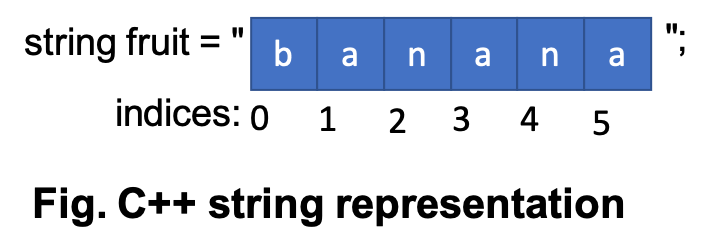
\includegraphics{resources/string_rep.png}

\hypertarget{c-string-example}{%
\subsubsection{C-string example}\label{c-string-example}}

\begin{itemize}
\tightlist
\item
  no need to include any library to use C-string
\end{itemize}

    \hypertarget{object-members}{%
\subsection{Object Members}\label{object-members}}

\begin{itemize}
\tightlist
\item
  there are some member variables and many membmer functions (called
  methods) available in string objects
\item
  a complete list is provided in this reference:
  https://en.cppreference.com/w/cpp/string/basic\_string
\item
  we'll go over some commonly used methods with examples in this
  notebook
\item
  syntax to access members of objects:
\end{itemize}

\begin{Shaded}
\begin{Highlighting}[]
\NormalTok{    object}\OperatorTok{.}\NormalTok{member\_variable}
\NormalTok{    object}\OperatorTok{.}\NormalTok{member\_function}\OperatorTok{()}
\end{Highlighting}
\end{Shaded}

\begin{itemize}
\tightlist
\item
  we use \texttt{.} (dot) member access operator to access object's
  members
\end{itemize}

    \hypertarget{element-access}{%
\subsection{Element access}\label{element-access}}

\begin{itemize}
\tightlist
\item
  extracting and updating characters
\item
  the following member functions/methods let's you access element:

  \begin{itemize}
  \tightlist
  \item
    \textbf{at(index)} - access the specified character at index with
    bounds checking
  \item
    \textbf{operator{[}index{]}} - access the specified character at
    index without bounds checking
  \item
    \textbf{front( )} - access the first character
  \item
    \textbf{back( )} - access the last character
  \end{itemize}
\item
  index must be a valid index between \textbf{0 to length-1}
\end{itemize}

    \begin{tcolorbox}[breakable, size=fbox, boxrule=1pt, pad at break*=1mm,colback=cellbackground, colframe=cellborder]
\prompt{In}{incolor}{35}{\boxspacing}
\begin{Verbatim}[commandchars=\\\{\}]
\PY{n}{string} \PY{n}{fruit} \PY{o}{=} \PY{l+s}{\PYZdq{}}\PY{l+s}{banana}\PY{l+s}{\PYZdq{}}\PY{p}{;}
\end{Verbatim}
\end{tcolorbox}

    \begin{tcolorbox}[breakable, size=fbox, boxrule=1pt, pad at break*=1mm,colback=cellbackground, colframe=cellborder]
\prompt{In}{incolor}{36}{\boxspacing}
\begin{Verbatim}[commandchars=\\\{\}]
\PY{k+kt}{char} \PY{n}{first\PYZus{}letter}\PY{p}{;}
\end{Verbatim}
\end{tcolorbox}

    \begin{tcolorbox}[breakable, size=fbox, boxrule=1pt, pad at break*=1mm,colback=cellbackground, colframe=cellborder]
\prompt{In}{incolor}{37}{\boxspacing}
\begin{Verbatim}[commandchars=\\\{\}]
\PY{c+c1}{// access the first character at index 0}
\PY{n}{first\PYZus{}letter} \PY{o}{=} \PY{n}{fruit}\PY{p}{.}\PY{n}{at}\PY{p}{(}\PY{l+m+mi}{0}\PY{p}{)}\PY{p}{;}
\end{Verbatim}
\end{tcolorbox}

    \begin{tcolorbox}[breakable, size=fbox, boxrule=1pt, pad at break*=1mm,colback=cellbackground, colframe=cellborder]
\prompt{In}{incolor}{38}{\boxspacing}
\begin{Verbatim}[commandchars=\\\{\}]
\PY{n}{cout} \PY{o}{\PYZlt{}}\PY{o}{\PYZlt{}} \PY{l+s}{\PYZdq{}}\PY{l+s}{first letter of }\PY{l+s}{\PYZdq{}} \PY{o}{\PYZlt{}}\PY{o}{\PYZlt{}} \PY{n}{fruit} \PY{o}{\PYZlt{}}\PY{o}{\PYZlt{}} \PY{l+s}{\PYZdq{}}\PY{l+s}{ is }\PY{l+s}{\PYZdq{}} \PY{o}{\PYZlt{}}\PY{o}{\PYZlt{}} \PY{n}{first\PYZus{}letter} \PY{o}{\PYZlt{}}\PY{o}{\PYZlt{}} \PY{l+s}{\PYZdq{}}\PY{l+s}{ = }\PY{l+s}{\PYZdq{}} \PY{o}{\PYZlt{}}\PY{o}{\PYZlt{}} \PY{n}{fruit}\PY{p}{[}\PY{l+m+mi}{0}\PY{p}{]}\PY{p}{;}
\end{Verbatim}
\end{tcolorbox}

    \begin{Verbatim}[commandchars=\\\{\}]
first letter of banana is b = b
    \end{Verbatim}

    \begin{tcolorbox}[breakable, size=fbox, boxrule=1pt, pad at break*=1mm,colback=cellbackground, colframe=cellborder]
\prompt{In}{incolor}{39}{\boxspacing}
\begin{Verbatim}[commandchars=\\\{\}]
\PY{c+c1}{//second character}
\PY{n}{cout} \PY{o}{\PYZlt{}}\PY{o}{\PYZlt{}} \PY{l+s}{\PYZdq{}}\PY{l+s}{second character = }\PY{l+s}{\PYZdq{}} \PY{o}{\PYZlt{}}\PY{o}{\PYZlt{}} \PY{n}{fruit}\PY{p}{[}\PY{l+m+mi}{1}\PY{p}{]} \PY{o}{\PYZlt{}}\PY{o}{\PYZlt{}} \PY{l+s}{\PYZdq{}}\PY{l+s}{ = }\PY{l+s}{\PYZdq{}} \PY{o}{\PYZlt{}}\PY{o}{\PYZlt{}} \PY{n}{fruit}\PY{p}{.}\PY{n}{at}\PY{p}{(}\PY{l+m+mi}{1}\PY{p}{)}\PY{p}{;}
\end{Verbatim}
\end{tcolorbox}

    \begin{Verbatim}[commandchars=\\\{\}]
second character = a = a
    \end{Verbatim}

    \begin{tcolorbox}[breakable, size=fbox, boxrule=1pt, pad at break*=1mm,colback=cellbackground, colframe=cellborder]
\prompt{In}{incolor}{ }{\boxspacing}
\begin{Verbatim}[commandchars=\\\{\}]
\PY{c+c1}{// there are 6 characters in banana}
\PY{n}{cout} \PY{o}{\PYZlt{}}\PY{o}{\PYZlt{}} \PY{l+s}{\PYZdq{}}\PY{l+s}{last character = }\PY{l+s}{\PYZdq{}} \PY{o}{\PYZlt{}}\PY{o}{\PYZlt{}} \PY{n}{fruit}\PY{p}{[}\PY{l+m+mi}{6}\PY{p}{]}\PY{p}{;}
\PY{c+c1}{// [] \PYZhy{} doesn\PYZsq{}t check the bound; output is undetermined}
\end{Verbatim}
\end{tcolorbox}

    \begin{tcolorbox}[breakable, size=fbox, boxrule=1pt, pad at break*=1mm,colback=cellbackground, colframe=cellborder]
\prompt{In}{incolor}{41}{\boxspacing}
\begin{Verbatim}[commandchars=\\\{\}]
\PY{c+c1}{// at() \PYZhy{} checks the bounds; throws runtime\PYZhy{}error}
\PY{n}{cout} \PY{o}{\PYZlt{}}\PY{o}{\PYZlt{}} \PY{l+s}{\PYZdq{}}\PY{l+s}{last character = }\PY{l+s}{\PYZdq{}} \PY{o}{\PYZlt{}}\PY{o}{\PYZlt{}} \PY{n}{fruit}\PY{p}{.}\PY{n}{at}\PY{p}{(}\PY{l+m+mi}{6}\PY{p}{)}\PY{p}{;}
\end{Verbatim}
\end{tcolorbox}

    \begin{Verbatim}[commandchars=\\\{\}]
last character =
    \end{Verbatim}

    \begin{Verbatim}[commandchars=\\\{\}, frame=single, framerule=2mm, rulecolor=\color{outerrorbackground}]
Standard Exception: basic\_string
    \end{Verbatim}

    \begin{tcolorbox}[breakable, size=fbox, boxrule=1pt, pad at break*=1mm,colback=cellbackground, colframe=cellborder]
\prompt{In}{incolor}{42}{\boxspacing}
\begin{Verbatim}[commandchars=\\\{\}]
\PY{n}{cout} \PY{o}{\PYZlt{}}\PY{o}{\PYZlt{}} \PY{l+s}{\PYZdq{}}\PY{l+s}{front = }\PY{l+s}{\PYZdq{}} \PY{o}{\PYZlt{}}\PY{o}{\PYZlt{}} \PY{n}{fruit}\PY{p}{.}\PY{n}{front}\PY{p}{(}\PY{p}{)} \PY{o}{\PYZlt{}}\PY{o}{\PYZlt{}} \PY{l+s}{\PYZdq{}}\PY{l+s}{ and back = }\PY{l+s}{\PYZdq{}} \PY{o}{\PYZlt{}}\PY{o}{\PYZlt{}} \PY{n}{fruit}\PY{p}{.}\PY{n}{back}\PY{p}{(}\PY{p}{)}\PY{p}{;}
\end{Verbatim}
\end{tcolorbox}

    \begin{Verbatim}[commandchars=\\\{\}]
front = b and back = a
    \end{Verbatim}

    \hypertarget{updating-string-in-place}{%
\subsubsection{Updating string in
place}\label{updating-string-in-place}}

\begin{itemize}
\tightlist
\item
  string is a mutable type that can be changed in place!
\item
  using \texttt{{[}\ \ {]}} - member access operator, we can assign new
  character at some index

  \begin{itemize}
  \tightlist
  \item
    index must be a valid one between \textbf{{[}0 \ldots{} length-1{]}}
  \end{itemize}
\end{itemize}

    \begin{tcolorbox}[breakable, size=fbox, boxrule=1pt, pad at break*=1mm,colback=cellbackground, colframe=cellborder]
\prompt{In}{incolor}{43}{\boxspacing}
\begin{Verbatim}[commandchars=\\\{\}]
\PY{c+c1}{// capitalize the first character by replacing \PYZsq{}b\PYZsq{} with \PYZsq{}B\PYZsq{}}
\PY{n}{fruit}\PY{p}{[}\PY{l+m+mi}{0}\PY{p}{]} \PY{o}{=} \PY{l+s+sc}{\PYZsq{}}\PY{l+s+sc}{B}\PY{l+s+sc}{\PYZsq{}}\PY{p}{;}
\end{Verbatim}
\end{tcolorbox}

    \begin{tcolorbox}[breakable, size=fbox, boxrule=1pt, pad at break*=1mm,colback=cellbackground, colframe=cellborder]
\prompt{In}{incolor}{44}{\boxspacing}
\begin{Verbatim}[commandchars=\\\{\}]
\PY{n}{cout} \PY{o}{\PYZlt{}}\PY{o}{\PYZlt{}} \PY{l+s}{\PYZdq{}}\PY{l+s}{I love, }\PY{l+s}{\PYZdq{}} \PY{o}{\PYZlt{}}\PY{o}{\PYZlt{}} \PY{n}{fruit} \PY{o}{\PYZlt{}}\PY{o}{\PYZlt{}} \PY{l+s}{\PYZdq{}}\PY{l+s}{!}\PY{l+s}{\PYZdq{}}\PY{p}{;}
\end{Verbatim}
\end{tcolorbox}

    \begin{Verbatim}[commandchars=\\\{\}]
I love, Banana!
    \end{Verbatim}

    \hypertarget{capacity}{%
\subsection{Capacity}\label{capacity}}

\begin{itemize}
\tightlist
\item
  knowing the length of a string (numbers of characters) helps with many
  operations
\item
  the following methods provide capacity of string objects:

  \begin{itemize}
  \tightlist
  \item
    \textbf{length()} or \textbf{size()} - returns the number of
    characters
  \item
    \textbf{empty()} - checks whether the string is empty
  \end{itemize}
\end{itemize}

    \begin{tcolorbox}[breakable, size=fbox, boxrule=1pt, pad at break*=1mm,colback=cellbackground, colframe=cellborder]
\prompt{In}{incolor}{45}{\boxspacing}
\begin{Verbatim}[commandchars=\\\{\}]
\PY{n}{cout} \PY{o}{\PYZlt{}}\PY{o}{\PYZlt{}} \PY{l+s}{\PYZdq{}}\PY{l+s}{length of }\PY{l+s}{\PYZdq{}} \PY{o}{\PYZlt{}}\PY{o}{\PYZlt{}} \PY{n}{fruit} \PY{o}{\PYZlt{}}\PY{o}{\PYZlt{}} \PY{l+s}{\PYZdq{}}\PY{l+s}{ = }\PY{l+s}{\PYZdq{}} \PY{o}{\PYZlt{}}\PY{o}{\PYZlt{}} \PY{n}{fruit}\PY{p}{.}\PY{n}{size}\PY{p}{(}\PY{p}{)} \PY{o}{\PYZlt{}}\PY{o}{\PYZlt{}} \PY{l+s}{\PYZdq{}}\PY{l+s}{ = }\PY{l+s}{\PYZdq{}} \PY{o}{\PYZlt{}}\PY{o}{\PYZlt{}} \PY{n}{fruit}\PY{p}{.}\PY{n}{length}\PY{p}{(}\PY{p}{)}\PY{p}{;}
\end{Verbatim}
\end{tcolorbox}

    \begin{Verbatim}[commandchars=\\\{\}]
length of Banana = 6 = 6
    \end{Verbatim}

    \begin{tcolorbox}[breakable, size=fbox, boxrule=1pt, pad at break*=1mm,colback=cellbackground, colframe=cellborder]
\prompt{In}{incolor}{48}{\boxspacing}
\begin{Verbatim}[commandchars=\\\{\}]
\PY{n}{cout} \PY{o}{\PYZlt{}}\PY{o}{\PYZlt{}} \PY{l+s}{\PYZdq{}}\PY{l+s}{is fruit empty? }\PY{l+s}{\PYZdq{}} \PY{o}{\PYZlt{}}\PY{o}{\PYZlt{}} \PY{n}{boolalpha} \PY{o}{\PYZlt{}}\PY{o}{\PYZlt{}} \PY{n}{fruit}\PY{p}{.}\PY{n}{empty}\PY{p}{(}\PY{p}{)}\PY{p}{;}
\end{Verbatim}
\end{tcolorbox}

    \begin{Verbatim}[commandchars=\\\{\}]
is fruit empty? false
    \end{Verbatim}

    \hypertarget{traversal}{%
\subsection{Traversal}\label{traversal}}

\begin{itemize}
\tightlist
\item
  traversing a string is a common task where you access every character
  from first to the last
\item
  there are several ways to traverse a string
\end{itemize}

    \begin{tcolorbox}[breakable, size=fbox, boxrule=1pt, pad at break*=1mm,colback=cellbackground, colframe=cellborder]
\prompt{In}{incolor}{96}{\boxspacing}
\begin{Verbatim}[commandchars=\\\{\}]
\PY{c+c1}{// using capacity to traverse/iterate over a string}
\PY{k}{for}\PY{p}{(}\PY{k+kt}{int} \PY{n}{i}\PY{o}{=}\PY{l+m+mi}{0}\PY{p}{;} \PY{n}{i}\PY{o}{\PYZlt{}}\PY{n}{fruit}\PY{p}{.}\PY{n}{length}\PY{p}{(}\PY{p}{)}\PY{p}{;} \PY{n}{i}\PY{o}{+}\PY{o}{+}\PY{p}{)} \PY{p}{\PYZob{}}
    \PY{n}{cout} \PY{o}{\PYZlt{}}\PY{o}{\PYZlt{}} \PY{l+s}{\PYZdq{}}\PY{l+s}{fruit[}\PY{l+s}{\PYZdq{}} \PY{o}{\PYZlt{}}\PY{o}{\PYZlt{}} \PY{n}{i} \PY{o}{\PYZlt{}}\PY{o}{\PYZlt{}} \PY{l+s}{\PYZdq{}}\PY{l+s}{] = }\PY{l+s}{\PYZdq{}} \PY{o}{\PYZlt{}}\PY{o}{\PYZlt{}} \PY{n}{fruit}\PY{p}{[}\PY{n}{i}\PY{p}{]} \PY{o}{\PYZlt{}}\PY{o}{\PYZlt{}} \PY{n}{endl}\PY{p}{;}
\PY{p}{\PYZcb{}}
\end{Verbatim}
\end{tcolorbox}

    \begin{Verbatim}[commandchars=\\\{\}]
fruit[0] = B
fruit[1] = a
fruit[2] = n
fruit[3] = a
fruit[4] = n
fruit[5] = a
    \end{Verbatim}

    \begin{tcolorbox}[breakable, size=fbox, boxrule=1pt, pad at break*=1mm,colback=cellbackground, colframe=cellborder]
\prompt{In}{incolor}{95}{\boxspacing}
\begin{Verbatim}[commandchars=\\\{\}]
\PY{c+cp}{\PYZsh{}}\PY{c+cp}{include} \PY{c+cpf}{\PYZlt{}cctype\PYZgt{}}

\PY{k}{for}\PY{p}{(}\PY{k}{auto} \PY{n+nl}{ch}\PY{p}{:} \PY{n}{fruit}\PY{p}{)}
    \PY{n}{cout} \PY{o}{\PYZlt{}}\PY{o}{\PYZlt{}} \PY{n}{ch} \PY{o}{\PYZlt{}}\PY{o}{\PYZlt{}} \PY{l+s}{\PYZdq{}}\PY{l+s}{ \PYZhy{}\PYZgt{} }\PY{l+s}{\PYZdq{}} \PY{o}{\PYZlt{}}\PY{o}{\PYZlt{}} \PY{k+kt}{char}\PY{p}{(}\PY{n}{toupper}\PY{p}{(}\PY{n}{ch}\PY{p}{)}\PY{p}{)} \PY{o}{\PYZlt{}}\PY{o}{\PYZlt{}} \PY{n}{endl}\PY{p}{;}
\end{Verbatim}
\end{tcolorbox}

    \begin{Verbatim}[commandchars=\\\{\}]
B -> B
a -> A
n -> N
a -> A
n -> N
a -> A
    \end{Verbatim}

    \hypertarget{iterators}{%
\subsection{Iterators}\label{iterators}}

\begin{itemize}
\tightlist
\item
  iterators are special pointers that let you iterate over or traverse a
  string
\item
  the following methods return an iterator:

  \begin{itemize}
  \tightlist
  \item
    \textbf{begin( )} - returns a forward iterator to the beginning
  \item
    \textbf{end( )} - returns a forward iterator to the end
  \item
    \textbf{rbegin( )} - returns a reverse iterator to the beginning
  \item
    \textbf{rend( )} - returns a reverse iterator to the end
  \end{itemize}
\item
  the following figure demonstrates begin() and end() iterators
\end{itemize}

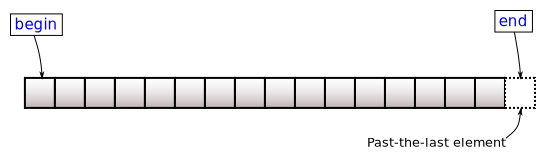
\includegraphics{resources/range-begin-end.png}

\begin{itemize}
\tightlist
\item
  the following figure demonstrates rbegin() and rend() iterators
\end{itemize}

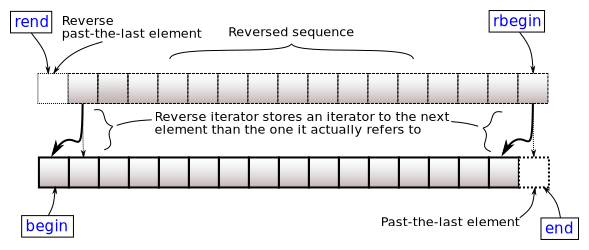
\includegraphics{resources/range-rbegin-rend.png}

    \begin{tcolorbox}[breakable, size=fbox, boxrule=1pt, pad at break*=1mm,colback=cellbackground, colframe=cellborder]
\prompt{In}{incolor}{20}{\boxspacing}
\begin{Verbatim}[commandchars=\\\{\}]
\PY{c+c1}{// automatically determine the type of iter which is a forward iterator}
\PY{k}{auto} \PY{n}{iter} \PY{o}{=} \PY{n}{fruit}\PY{p}{.}\PY{n}{begin}\PY{p}{(}\PY{p}{)}\PY{p}{;}
\end{Verbatim}
\end{tcolorbox}

    \begin{tcolorbox}[breakable, size=fbox, boxrule=1pt, pad at break*=1mm,colback=cellbackground, colframe=cellborder]
\prompt{In}{incolor}{21}{\boxspacing}
\begin{Verbatim}[commandchars=\\\{\}]
\PY{c+c1}{// what is iter pointing to?}
\PY{n}{cout} \PY{o}{\PYZlt{}}\PY{o}{\PYZlt{}} \PY{o}{*}\PY{n}{iter}\PY{p}{;}
\end{Verbatim}
\end{tcolorbox}

    \begin{Verbatim}[commandchars=\\\{\}]
B
    \end{Verbatim}

    \begin{tcolorbox}[breakable, size=fbox, boxrule=1pt, pad at break*=1mm,colback=cellbackground, colframe=cellborder]
\prompt{In}{incolor}{22}{\boxspacing}
\begin{Verbatim}[commandchars=\\\{\}]
\PY{c+c1}{// increment iterator by one element}
\PY{n}{iter} \PY{o}{+}\PY{o}{=} \PY{l+m+mi}{1}\PY{p}{;}
\end{Verbatim}
\end{tcolorbox}

    \begin{tcolorbox}[breakable, size=fbox, boxrule=1pt, pad at break*=1mm,colback=cellbackground, colframe=cellborder]
\prompt{In}{incolor}{23}{\boxspacing}
\begin{Verbatim}[commandchars=\\\{\}]
\PY{n}{cout} \PY{o}{\PYZlt{}}\PY{o}{\PYZlt{}} \PY{o}{*}\PY{n}{iter}\PY{p}{;}
\end{Verbatim}
\end{tcolorbox}

    \begin{Verbatim}[commandchars=\\\{\}]
a
    \end{Verbatim}

    \begin{tcolorbox}[breakable, size=fbox, boxrule=1pt, pad at break*=1mm,colback=cellbackground, colframe=cellborder]
\prompt{In}{incolor}{24}{\boxspacing}
\begin{Verbatim}[commandchars=\\\{\}]
\PY{c+c1}{// forward iterator}
\PY{k}{for}\PY{p}{(}\PY{k}{auto} \PY{n}{it}\PY{o}{=}\PY{n}{fruit}\PY{p}{.}\PY{n}{begin}\PY{p}{(}\PY{p}{)}\PY{p}{;} \PY{n}{it} \PY{o}{!}\PY{o}{=} \PY{n}{fruit}\PY{p}{.}\PY{n}{end}\PY{p}{(}\PY{p}{)}\PY{p}{;} \PY{n}{it} \PY{o}{+}\PY{o}{=} \PY{l+m+mi}{1}\PY{p}{)} \PY{p}{\PYZob{}}
    \PY{n}{cout} \PY{o}{\PYZlt{}}\PY{o}{\PYZlt{}} \PY{o}{*}\PY{n}{it} \PY{o}{\PYZlt{}}\PY{o}{\PYZlt{}} \PY{l+s}{\PYZdq{}}\PY{l+s}{ }\PY{l+s}{\PYZdq{}}\PY{p}{;}
\PY{p}{\PYZcb{}}
\end{Verbatim}
\end{tcolorbox}

    \begin{Verbatim}[commandchars=\\\{\}]
B a n a n a
    \end{Verbatim}

    \begin{tcolorbox}[breakable, size=fbox, boxrule=1pt, pad at break*=1mm,colback=cellbackground, colframe=cellborder]
\prompt{In}{incolor}{25}{\boxspacing}
\begin{Verbatim}[commandchars=\\\{\}]
\PY{c+c1}{// reverse iterator}
\PY{k}{for}\PY{p}{(}\PY{k}{auto} \PY{n}{it}\PY{o}{=}\PY{n}{fruit}\PY{p}{.}\PY{n}{rbegin}\PY{p}{(}\PY{p}{)}\PY{p}{;} \PY{n}{it}\PY{o}{!}\PY{o}{=}\PY{n}{fruit}\PY{p}{.}\PY{n}{rend}\PY{p}{(}\PY{p}{)}\PY{p}{;} \PY{n}{it}\PY{o}{+}\PY{o}{+}\PY{p}{)} \PY{p}{\PYZob{}}
    \PY{n}{cout} \PY{o}{\PYZlt{}}\PY{o}{\PYZlt{}} \PY{o}{*}\PY{n}{it} \PY{o}{\PYZlt{}}\PY{o}{\PYZlt{}} \PY{l+s}{\PYZdq{}}\PY{l+s}{ }\PY{l+s}{\PYZdq{}}\PY{p}{;}
\PY{p}{\PYZcb{}}
\end{Verbatim}
\end{tcolorbox}

    \begin{Verbatim}[commandchars=\\\{\}]
a n a n a B
    \end{Verbatim}

    \hypertarget{operations}{%
\subsection{Operations}\label{operations}}

\begin{itemize}
\tightlist
\item
  string objects have a bunch of methods to perform various common
  operations on string data
\item
  the following are some commonly used operations:
\end{itemize}

    \hypertarget{clear}{%
\subsubsection{clear}\label{clear}}

\begin{itemize}
\tightlist
\item
  clears the contents making string object empty!
\end{itemize}

    \begin{tcolorbox}[breakable, size=fbox, boxrule=1pt, pad at break*=1mm,colback=cellbackground, colframe=cellborder]
\prompt{In}{incolor}{4}{\boxspacing}
\begin{Verbatim}[commandchars=\\\{\}]
\PY{n}{string} \PY{n}{strData} \PY{o}{=} \PY{l+s}{\PYZdq{}}\PY{l+s}{Pirates of the Carribean!}\PY{l+s}{\PYZdq{}}\PY{p}{;}
\end{Verbatim}
\end{tcolorbox}

    \begin{tcolorbox}[breakable, size=fbox, boxrule=1pt, pad at break*=1mm,colback=cellbackground, colframe=cellborder]
\prompt{In}{incolor}{5}{\boxspacing}
\begin{Verbatim}[commandchars=\\\{\}]
\PY{c+c1}{// clear the content}
\PY{n}{strData}\PY{p}{.}\PY{n}{clear}\PY{p}{(}\PY{p}{)}\PY{p}{;}
\PY{n}{cout} \PY{o}{\PYZlt{}}\PY{o}{\PYZlt{}} \PY{l+s}{\PYZdq{}}\PY{l+s}{strData = }\PY{l+s}{\PYZdq{}} \PY{o}{\PYZlt{}}\PY{o}{\PYZlt{}} \PY{n}{strData}\PY{p}{;}
\end{Verbatim}
\end{tcolorbox}

    \begin{Verbatim}[commandchars=\\\{\}]
strData =
    \end{Verbatim}

    \hypertarget{insert}{%
\subsubsection{insert}\label{insert}}

\begin{itemize}
\tightlist
\item
  insert a character or string at some given index
\item
  \textbf{insert(index, count, char)} insert \texttt{count}
  \texttt{char}acters at some \texttt{index}
\item
  \textbf{insert(index, string)} - insert some \texttt{string} at
  \texttt{index}
\end{itemize}

    \begin{tcolorbox}[breakable, size=fbox, boxrule=1pt, pad at break*=1mm,colback=cellbackground, colframe=cellborder]
\prompt{In}{incolor}{5}{\boxspacing}
\begin{Verbatim}[commandchars=\\\{\}]
\PY{n}{strData} \PY{o}{=} \PY{l+s}{\PYZdq{}}\PY{l+s}{Pirates of the Carribean!}\PY{l+s}{\PYZdq{}}\PY{p}{;}
\end{Verbatim}
\end{tcolorbox}

    \begin{tcolorbox}[breakable, size=fbox, boxrule=1pt, pad at break*=1mm,colback=cellbackground, colframe=cellborder]
\prompt{In}{incolor}{7}{\boxspacing}
\begin{Verbatim}[commandchars=\\\{\}]
\PY{c+c1}{// insert 1 \PYZdl{} at index 0}
\PY{n}{strData}\PY{p}{.}\PY{n}{insert}\PY{p}{(}\PY{l+m+mi}{0}\PY{p}{,} \PY{l+m+mi}{1}\PY{p}{,} \PY{l+s+sc}{\PYZsq{}}\PY{l+s+sc}{\PYZdl{}}\PY{l+s+sc}{\PYZsq{}}\PY{p}{)}\PY{p}{;}
\end{Verbatim}
\end{tcolorbox}

    \begin{tcolorbox}[breakable, size=fbox, boxrule=1pt, pad at break*=1mm,colback=cellbackground, colframe=cellborder]
\prompt{In}{incolor}{8}{\boxspacing}
\begin{Verbatim}[commandchars=\\\{\}]
\PY{n}{cout} \PY{o}{\PYZlt{}}\PY{o}{\PYZlt{}} \PY{l+s}{\PYZdq{}}\PY{l+s}{strData = }\PY{l+s}{\PYZdq{}} \PY{o}{\PYZlt{}}\PY{o}{\PYZlt{}} \PY{n}{strData}\PY{p}{;}
\end{Verbatim}
\end{tcolorbox}

    \begin{Verbatim}[commandchars=\\\{\}]
strData = \$Pirates of the Carribean!
    \end{Verbatim}

    \begin{tcolorbox}[breakable, size=fbox, boxrule=1pt, pad at break*=1mm,colback=cellbackground, colframe=cellborder]
\prompt{In}{incolor}{10}{\boxspacing}
\begin{Verbatim}[commandchars=\\\{\}]
\PY{c+c1}{// insert 5 astersisks at index 5}
\PY{n}{strData}\PY{p}{.}\PY{n}{insert}\PY{p}{(}\PY{l+m+mi}{5}\PY{p}{,} \PY{l+m+mi}{5}\PY{p}{,} \PY{l+s+sc}{\PYZsq{}}\PY{l+s+sc}{*}\PY{l+s+sc}{\PYZsq{}}\PY{p}{)}\PY{p}{;}
\end{Verbatim}
\end{tcolorbox}

    \begin{tcolorbox}[breakable, size=fbox, boxrule=1pt, pad at break*=1mm,colback=cellbackground, colframe=cellborder]
\prompt{In}{incolor}{11}{\boxspacing}
\begin{Verbatim}[commandchars=\\\{\}]
\PY{n}{cout} \PY{o}{\PYZlt{}}\PY{o}{\PYZlt{}} \PY{l+s}{\PYZdq{}}\PY{l+s}{strData = }\PY{l+s}{\PYZdq{}} \PY{o}{\PYZlt{}}\PY{o}{\PYZlt{}} \PY{n}{strData}\PY{p}{;}
\end{Verbatim}
\end{tcolorbox}

    \begin{Verbatim}[commandchars=\\\{\}]
strData = \$Pira*****tes of the Carribean!
    \end{Verbatim}

    \begin{tcolorbox}[breakable, size=fbox, boxrule=1pt, pad at break*=1mm,colback=cellbackground, colframe=cellborder]
\prompt{In}{incolor}{12}{\boxspacing}
\begin{Verbatim}[commandchars=\\\{\}]
\PY{n}{strData}\PY{p}{.}\PY{n}{insert}\PY{p}{(}\PY{l+m+mi}{0}\PY{p}{,} \PY{l+s}{\PYZdq{}}\PY{l+s}{The }\PY{l+s}{\PYZdq{}}\PY{p}{)}\PY{p}{;}
\end{Verbatim}
\end{tcolorbox}

    \begin{tcolorbox}[breakable, size=fbox, boxrule=1pt, pad at break*=1mm,colback=cellbackground, colframe=cellborder]
\prompt{In}{incolor}{13}{\boxspacing}
\begin{Verbatim}[commandchars=\\\{\}]
\PY{n}{cout} \PY{o}{\PYZlt{}}\PY{o}{\PYZlt{}} \PY{l+s}{\PYZdq{}}\PY{l+s}{strData = }\PY{l+s}{\PYZdq{}} \PY{o}{\PYZlt{}}\PY{o}{\PYZlt{}} \PY{n}{strData}\PY{p}{;}
\end{Verbatim}
\end{tcolorbox}

    \begin{Verbatim}[commandchars=\\\{\}]
strData = The \$Pira*****tes of the Carribean!
    \end{Verbatim}

    \hypertarget{erase}{%
\subsubsection{erase}\label{erase}}

\textbf{erase(index, count)} - erases \texttt{count} characters starting
from \texttt{index}

    \begin{tcolorbox}[breakable, size=fbox, boxrule=1pt, pad at break*=1mm,colback=cellbackground, colframe=cellborder]
\prompt{In}{incolor}{14}{\boxspacing}
\begin{Verbatim}[commandchars=\\\{\}]
\PY{c+c1}{// erase all 5 asterisks starting at index 9}
\PY{n}{strData}\PY{p}{.}\PY{n}{erase}\PY{p}{(}\PY{l+m+mi}{9}\PY{p}{,} \PY{l+m+mi}{5}\PY{p}{)}\PY{p}{;}
\end{Verbatim}
\end{tcolorbox}

    \begin{tcolorbox}[breakable, size=fbox, boxrule=1pt, pad at break*=1mm,colback=cellbackground, colframe=cellborder]
\prompt{In}{incolor}{15}{\boxspacing}
\begin{Verbatim}[commandchars=\\\{\}]
\PY{n}{strData}
\end{Verbatim}
\end{tcolorbox}

            \begin{tcolorbox}[breakable, size=fbox, boxrule=.5pt, pad at break*=1mm, opacityfill=0]
\prompt{Out}{outcolor}{15}{\boxspacing}
\begin{Verbatim}[commandchars=\\\{\}]
"The \$Pirates of the Carribean!"
\end{Verbatim}
\end{tcolorbox}
        
    \hypertarget{append}{%
\subsubsection{append}\label{append}}

\begin{itemize}
\tightlist
\item
  the following methods append characters to the end of string objects

  \begin{itemize}
  \tightlist
  \item
    \textbf{push\_back(ch)} - appends a character to the end
  \item
    \textbf{append(str)} - appends string to the end
  \item
    \textbf{operator+=} - appends string to the end
  \end{itemize}
\end{itemize}

    \begin{tcolorbox}[breakable, size=fbox, boxrule=1pt, pad at break*=1mm,colback=cellbackground, colframe=cellborder]
\prompt{In}{incolor}{3}{\boxspacing}
\begin{Verbatim}[commandchars=\\\{\}]
\PY{n}{string} \PY{n}{some\PYZus{}str}\PY{p}{;}
\end{Verbatim}
\end{tcolorbox}

    \begin{tcolorbox}[breakable, size=fbox, boxrule=1pt, pad at break*=1mm,colback=cellbackground, colframe=cellborder]
\prompt{In}{incolor}{4}{\boxspacing}
\begin{Verbatim}[commandchars=\\\{\}]
\PY{n}{some\PYZus{}str} \PY{o}{=} \PY{l+s}{\PYZdq{}}\PY{l+s}{\PYZdq{}}\PY{p}{;}
\end{Verbatim}
\end{tcolorbox}

    \begin{tcolorbox}[breakable, size=fbox, boxrule=1pt, pad at break*=1mm,colback=cellbackground, colframe=cellborder]
\prompt{In}{incolor}{5}{\boxspacing}
\begin{Verbatim}[commandchars=\\\{\}]
\PY{n}{some\PYZus{}str}\PY{p}{.}\PY{n}{push\PYZus{}back}\PY{p}{(}\PY{l+s+sc}{\PYZsq{}}\PY{l+s+sc}{1}\PY{l+s+sc}{\PYZsq{}}\PY{p}{)}\PY{p}{;}
\PY{n}{some\PYZus{}str}\PY{p}{.}\PY{n}{append}\PY{p}{(}\PY{l+s}{\PYZdq{}}\PY{l+s}{2}\PY{l+s}{\PYZdq{}}\PY{p}{)}\PY{p}{;}
\PY{n}{some\PYZus{}str} \PY{o}{+}\PY{o}{=} \PY{l+s}{\PYZdq{}}\PY{l+s}{3456}\PY{l+s}{\PYZdq{}}\PY{p}{;}
\end{Verbatim}
\end{tcolorbox}

    \begin{tcolorbox}[breakable, size=fbox, boxrule=1pt, pad at break*=1mm,colback=cellbackground, colframe=cellborder]
\prompt{In}{incolor}{6}{\boxspacing}
\begin{Verbatim}[commandchars=\\\{\}]
\PY{n}{some\PYZus{}str}
\end{Verbatim}
\end{tcolorbox}

            \begin{tcolorbox}[breakable, size=fbox, boxrule=.5pt, pad at break*=1mm, opacityfill=0]
\prompt{Out}{outcolor}{6}{\boxspacing}
\begin{Verbatim}[commandchars=\\\{\}]
"123456"
\end{Verbatim}
\end{tcolorbox}
        
    \hypertarget{search}{%
\subsection{Search}\label{search}}

\begin{itemize}
\tightlist
\item
  searching for a substring is often a common task performed with
  strings data
\item
  also refered to as ``finding a needle in the haystack''
\item
  \texttt{find} and \texttt{rfind} methods help in finding a substring
  in some string
\end{itemize}

\hypertarget{find-str-pos}{%
\subsubsection{find( str, {[}pos{]} )}\label{find-str-pos}}

\begin{itemize}
\tightlist
\item
  finds the first \texttt{str} in the string starting from \texttt{pos}

  \begin{itemize}
  \tightlist
  \item
    if no \texttt{pos} is provided, first index, 0 is used
  \end{itemize}
\item
  if \texttt{str} is found, returns begining position/index of
  \texttt{str}
\item
  if str is not found, returns \texttt{npos} constant defined in
  \texttt{string::} namespace

  \begin{itemize}
  \tightlist
  \item
    \texttt{npos} is the largest possible value for \textbf{size\_t};
    system dependent
  \end{itemize}
\end{itemize}

    \begin{tcolorbox}[breakable, size=fbox, boxrule=1pt, pad at break*=1mm,colback=cellbackground, colframe=cellborder]
\prompt{In}{incolor}{7}{\boxspacing}
\begin{Verbatim}[commandchars=\\\{\}]
\PY{c+c1}{// what is npos?}
\PY{n}{cout} \PY{o}{\PYZlt{}}\PY{o}{\PYZlt{}} \PY{n}{string}\PY{o}{:}\PY{o}{:}\PY{n}{npos}\PY{p}{;}
\end{Verbatim}
\end{tcolorbox}

    \begin{Verbatim}[commandchars=\\\{\}]
18446744073709551615
    \end{Verbatim}

    \begin{tcolorbox}[breakable, size=fbox, boxrule=1pt, pad at break*=1mm,colback=cellbackground, colframe=cellborder]
\prompt{In}{incolor}{8}{\boxspacing}
\begin{Verbatim}[commandchars=\\\{\}]
\PY{n}{string} \PY{n}{haystack}\PY{p}{,} \PY{n}{search\PYZus{}str}\PY{p}{;}
\PY{k+kt}{size\PYZus{}t} \PY{n}{found}\PY{p}{;}
\end{Verbatim}
\end{tcolorbox}

    \begin{tcolorbox}[breakable, size=fbox, boxrule=1pt, pad at break*=1mm,colback=cellbackground, colframe=cellborder]
\prompt{In}{incolor}{9}{\boxspacing}
\begin{Verbatim}[commandchars=\\\{\}]
\PY{n}{haystack} \PY{o}{=} \PY{l+s}{\PYZdq{}}\PY{l+s}{There are maanny needles or just a few needle in the haystack!}\PY{l+s}{\PYZdq{}}\PY{p}{;}
\end{Verbatim}
\end{tcolorbox}

    \begin{tcolorbox}[breakable, size=fbox, boxrule=1pt, pad at break*=1mm,colback=cellbackground, colframe=cellborder]
\prompt{In}{incolor}{10}{\boxspacing}
\begin{Verbatim}[commandchars=\\\{\}]
\PY{n}{search\PYZus{}str} \PY{o}{=} \PY{l+s}{\PYZdq{}}\PY{l+s}{needle}\PY{l+s}{\PYZdq{}}\PY{p}{;} \PY{c+c1}{// TODO: change this to \PYZdq{}Needle\PYZdq{} and find}
\end{Verbatim}
\end{tcolorbox}

            \begin{tcolorbox}[breakable, size=fbox, boxrule=.5pt, pad at break*=1mm, opacityfill=0]
\prompt{Out}{outcolor}{10}{\boxspacing}
\begin{Verbatim}[commandchars=\\\{\}]
"needle"
\end{Verbatim}
\end{tcolorbox}
        
    \begin{tcolorbox}[breakable, size=fbox, boxrule=1pt, pad at break*=1mm,colback=cellbackground, colframe=cellborder]
\prompt{In}{incolor}{11}{\boxspacing}
\begin{Verbatim}[commandchars=\\\{\}]
\PY{n}{found} \PY{o}{=} \PY{n}{haystack}\PY{p}{.}\PY{n}{find}\PY{p}{(}\PY{n}{search\PYZus{}str}\PY{p}{)}\PY{p}{;}
\end{Verbatim}
\end{tcolorbox}

    \begin{tcolorbox}[breakable, size=fbox, boxrule=1pt, pad at break*=1mm,colback=cellbackground, colframe=cellborder]
\prompt{In}{incolor}{12}{\boxspacing}
\begin{Verbatim}[commandchars=\\\{\}]
\PY{n}{cout} \PY{o}{\PYZlt{}}\PY{o}{\PYZlt{}} \PY{n}{found}\PY{p}{;}
\end{Verbatim}
\end{tcolorbox}

    \begin{Verbatim}[commandchars=\\\{\}]
17
    \end{Verbatim}

    \begin{tcolorbox}[breakable, size=fbox, boxrule=1pt, pad at break*=1mm,colback=cellbackground, colframe=cellborder]
\prompt{In}{incolor}{13}{\boxspacing}
\begin{Verbatim}[commandchars=\\\{\}]
\PY{c+c1}{// check if substring is found or not}
\PY{k}{if} \PY{p}{(}\PY{n}{found} \PY{o}{=}\PY{o}{=} \PY{n}{string}\PY{o}{:}\PY{o}{:}\PY{n}{npos}\PY{p}{)}
    \PY{n}{cout} \PY{o}{\PYZlt{}}\PY{o}{\PYZlt{}} \PY{n}{search\PYZus{}str} \PY{o}{\PYZlt{}}\PY{o}{\PYZlt{}} \PY{l+s}{\PYZdq{}}\PY{l+s}{ NOT found!}\PY{l+s+se}{\PYZbs{}n}\PY{l+s}{\PYZdq{}}\PY{p}{;}
\PY{k}{else}
    \PY{n}{cout} \PY{o}{\PYZlt{}}\PY{o}{\PYZlt{}} \PY{n}{search\PYZus{}str} \PY{o}{\PYZlt{}}\PY{o}{\PYZlt{}} \PY{l+s}{\PYZdq{}}\PY{l+s}{ found at: }\PY{l+s}{\PYZdq{}} \PY{o}{\PYZlt{}}\PY{o}{\PYZlt{}} \PY{n}{found} \PY{o}{\PYZlt{}}\PY{o}{\PYZlt{}} \PY{n}{endl}\PY{p}{;}
\end{Verbatim}
\end{tcolorbox}

    \begin{Verbatim}[commandchars=\\\{\}]
needle found at: 17
    \end{Verbatim}

    \hypertarget{rfind-str-pos}{%
\subsubsection{rfind( str, {[}pos{]} )}\label{rfind-str-pos}}

\begin{itemize}
\tightlist
\item
  search the first substring in backward direction starting from
  \texttt{pos}

  \begin{itemize}
  \tightlist
  \item
    if no \texttt{pos} is provided, last index is used
  \end{itemize}
\end{itemize}

    \begin{tcolorbox}[breakable, size=fbox, boxrule=1pt, pad at break*=1mm,colback=cellbackground, colframe=cellborder]
\prompt{In}{incolor}{14}{\boxspacing}
\begin{Verbatim}[commandchars=\\\{\}]
\PY{n}{found} \PY{o}{=} \PY{n}{haystack}\PY{p}{.}\PY{n}{rfind}\PY{p}{(}\PY{n}{search\PYZus{}str}\PY{p}{)}\PY{p}{;}
\PY{c+c1}{// check if substring is found or not}
\PY{k}{if} \PY{p}{(}\PY{n}{found} \PY{o}{=}\PY{o}{=} \PY{n}{string}\PY{o}{:}\PY{o}{:}\PY{n}{npos}\PY{p}{)}
    \PY{n}{cout} \PY{o}{\PYZlt{}}\PY{o}{\PYZlt{}} \PY{n}{search\PYZus{}str} \PY{o}{\PYZlt{}}\PY{o}{\PYZlt{}} \PY{l+s}{\PYZdq{}}\PY{l+s}{ NOT found!}\PY{l+s+se}{\PYZbs{}n}\PY{l+s}{\PYZdq{}}\PY{p}{;}
\PY{k}{else}
    \PY{n}{cout} \PY{o}{\PYZlt{}}\PY{o}{\PYZlt{}} \PY{n}{search\PYZus{}str} \PY{o}{\PYZlt{}}\PY{o}{\PYZlt{}} \PY{l+s}{\PYZdq{}}\PY{l+s}{ found at: }\PY{l+s}{\PYZdq{}} \PY{o}{\PYZlt{}}\PY{o}{\PYZlt{}} \PY{n}{found} \PY{o}{\PYZlt{}}\PY{o}{\PYZlt{}} \PY{n}{endl}\PY{p}{;}
\end{Verbatim}
\end{tcolorbox}

    \begin{Verbatim}[commandchars=\\\{\}]
needle found at: 39
    \end{Verbatim}

    \hypertarget{replace}{%
\subsubsection{replace}\label{replace}}

\begin{itemize}
\tightlist
\item
  replaces the part of string indicated by \texttt{index} with a new
  string
\item
  \textbf{replace(index, count, newStr)}

  \begin{itemize}
  \tightlist
  \item
    replace some string from \texttt{index} to \texttt{index+count} by
    \texttt{newStr}
  \end{itemize}
\end{itemize}

    \begin{tcolorbox}[breakable, size=fbox, boxrule=1pt, pad at break*=1mm,colback=cellbackground, colframe=cellborder]
\prompt{In}{incolor}{15}{\boxspacing}
\begin{Verbatim}[commandchars=\\\{\}]
\PY{n}{some\PYZus{}str} \PY{o}{=} \PY{l+s}{\PYZdq{}}\PY{l+s}{12345abc}\PY{l+s}{\PYZdq{}}\PY{p}{;}
\end{Verbatim}
\end{tcolorbox}

    \begin{tcolorbox}[breakable, size=fbox, boxrule=1pt, pad at break*=1mm,colback=cellbackground, colframe=cellborder]
\prompt{In}{incolor}{16}{\boxspacing}
\begin{Verbatim}[commandchars=\\\{\}]
\PY{n}{some\PYZus{}str}\PY{p}{.}\PY{n}{replace}\PY{p}{(}\PY{l+m+mi}{0}\PY{p}{,} \PY{l+m+mi}{1}\PY{p}{,} \PY{l+s}{\PYZdq{}}\PY{l+s}{A}\PY{l+s}{\PYZdq{}}\PY{p}{)}\PY{p}{;}
\end{Verbatim}
\end{tcolorbox}

    \begin{tcolorbox}[breakable, size=fbox, boxrule=1pt, pad at break*=1mm,colback=cellbackground, colframe=cellborder]
\prompt{In}{incolor}{17}{\boxspacing}
\begin{Verbatim}[commandchars=\\\{\}]
\PY{n}{some\PYZus{}str}
\end{Verbatim}
\end{tcolorbox}

            \begin{tcolorbox}[breakable, size=fbox, boxrule=.5pt, pad at break*=1mm, opacityfill=0]
\prompt{Out}{outcolor}{17}{\boxspacing}
\begin{Verbatim}[commandchars=\\\{\}]
"A2345abc"
\end{Verbatim}
\end{tcolorbox}
        
    \begin{tcolorbox}[breakable, size=fbox, boxrule=1pt, pad at break*=1mm,colback=cellbackground, colframe=cellborder]
\prompt{In}{incolor}{18}{\boxspacing}
\begin{Verbatim}[commandchars=\\\{\}]
\PY{n}{some\PYZus{}str}\PY{p}{.}\PY{n}{replace}\PY{p}{(}\PY{l+m+mi}{1}\PY{p}{,} \PY{l+m+mi}{5}\PY{p}{,} \PY{l+s}{\PYZdq{}}\PY{l+s}{B}\PY{l+s}{\PYZdq{}}\PY{p}{)}\PY{p}{;}
\end{Verbatim}
\end{tcolorbox}

    \begin{tcolorbox}[breakable, size=fbox, boxrule=1pt, pad at break*=1mm,colback=cellbackground, colframe=cellborder]
\prompt{In}{incolor}{19}{\boxspacing}
\begin{Verbatim}[commandchars=\\\{\}]
\PY{n}{some\PYZus{}str}
\end{Verbatim}
\end{tcolorbox}

            \begin{tcolorbox}[breakable, size=fbox, boxrule=.5pt, pad at break*=1mm, opacityfill=0]
\prompt{Out}{outcolor}{19}{\boxspacing}
\begin{Verbatim}[commandchars=\\\{\}]
"ABbc"
\end{Verbatim}
\end{tcolorbox}
        
    \begin{tcolorbox}[breakable, size=fbox, boxrule=1pt, pad at break*=1mm,colback=cellbackground, colframe=cellborder]
\prompt{In}{incolor}{20}{\boxspacing}
\begin{Verbatim}[commandchars=\\\{\}]
\PY{c+c1}{// insert with replacing 0 character}
\PY{n}{some\PYZus{}str}\PY{p}{.}\PY{n}{replace}\PY{p}{(}\PY{l+m+mi}{1}\PY{p}{,} \PY{l+m+mi}{0}\PY{p}{,} \PY{l+s}{\PYZdq{}}\PY{l+s}{WXYZ}\PY{l+s}{\PYZdq{}}\PY{p}{)}\PY{p}{;}
\end{Verbatim}
\end{tcolorbox}

    \begin{tcolorbox}[breakable, size=fbox, boxrule=1pt, pad at break*=1mm,colback=cellbackground, colframe=cellborder]
\prompt{In}{incolor}{21}{\boxspacing}
\begin{Verbatim}[commandchars=\\\{\}]
\PY{n}{some\PYZus{}str}
\end{Verbatim}
\end{tcolorbox}

            \begin{tcolorbox}[breakable, size=fbox, boxrule=.5pt, pad at break*=1mm, opacityfill=0]
\prompt{Out}{outcolor}{21}{\boxspacing}
\begin{Verbatim}[commandchars=\\\{\}]
"AWXYZBbc"
\end{Verbatim}
\end{tcolorbox}
        
    \hypertarget{search-and-replace-application}{%
\subsubsection{Search and replace
application}\label{search-and-replace-application}}

\begin{itemize}
\tightlist
\item
  a commmon feature provided by text editors
\end{itemize}

    \begin{tcolorbox}[breakable, size=fbox, boxrule=1pt, pad at break*=1mm,colback=cellbackground, colframe=cellborder]
\prompt{In}{incolor}{23}{\boxspacing}
\begin{Verbatim}[commandchars=\\\{\}]
\PY{c+c1}{// let\PYZsq{}s see the contents of haystack}
\PY{n}{haystack}
\end{Verbatim}
\end{tcolorbox}

            \begin{tcolorbox}[breakable, size=fbox, boxrule=.5pt, pad at break*=1mm, opacityfill=0]
\prompt{Out}{outcolor}{23}{\boxspacing}
\begin{Verbatim}[commandchars=\\\{\}]
"There are maanny needles or just a few needle in the haystack!"
\end{Verbatim}
\end{tcolorbox}
        
    \begin{tcolorbox}[breakable, size=fbox, boxrule=1pt, pad at break*=1mm,colback=cellbackground, colframe=cellborder]
\prompt{In}{incolor}{28}{\boxspacing}
\begin{Verbatim}[commandchars=\\\{\}]
\PY{c+c1}{// let\PYZsq{}s search misspelled word \PYZdq{}maanny\PYZdq{} and replace with \PYZdq{}many\PYZdq{}}
\PY{k+kt}{size\PYZus{}t} \PY{n}{wordIndex} \PY{o}{=} \PY{n}{haystack}\PY{p}{.}\PY{n}{find}\PY{p}{(}\PY{l+s}{\PYZdq{}}\PY{l+s}{maanny}\PY{l+s}{\PYZdq{}}\PY{p}{)}
\end{Verbatim}
\end{tcolorbox}

    \begin{tcolorbox}[breakable, size=fbox, boxrule=1pt, pad at break*=1mm,colback=cellbackground, colframe=cellborder]
\prompt{In}{incolor}{29}{\boxspacing}
\begin{Verbatim}[commandchars=\\\{\}]
\PY{n}{wordIndex}
\end{Verbatim}
\end{tcolorbox}

            \begin{tcolorbox}[breakable, size=fbox, boxrule=.5pt, pad at break*=1mm, opacityfill=0]
\prompt{Out}{outcolor}{29}{\boxspacing}
\begin{Verbatim}[commandchars=\\\{\}]
10
\end{Verbatim}
\end{tcolorbox}
        
    \begin{tcolorbox}[breakable, size=fbox, boxrule=1pt, pad at break*=1mm,colback=cellbackground, colframe=cellborder]
\prompt{In}{incolor}{31}{\boxspacing}
\begin{Verbatim}[commandchars=\\\{\}]
\PY{n}{haystack}\PY{p}{.}\PY{n}{replace}\PY{p}{(}\PY{n}{wordIndex}\PY{p}{,} \PY{n}{string}\PY{p}{(}\PY{l+s}{\PYZdq{}}\PY{l+s}{maanny}\PY{l+s}{\PYZdq{}}\PY{p}{)}\PY{p}{.}\PY{n}{length}\PY{p}{(}\PY{p}{)}\PY{p}{,} \PY{l+s}{\PYZdq{}}\PY{l+s}{many}\PY{l+s}{\PYZdq{}}\PY{p}{)}
\end{Verbatim}
\end{tcolorbox}

            \begin{tcolorbox}[breakable, size=fbox, boxrule=.5pt, pad at break*=1mm, opacityfill=0]
\prompt{Out}{outcolor}{31}{\boxspacing}
\begin{Verbatim}[commandchars=\\\{\}]
"There are many needles or just a few needle in the haystack!"
\end{Verbatim}
\end{tcolorbox}
        
    \begin{tcolorbox}[breakable, size=fbox, boxrule=1pt, pad at break*=1mm,colback=cellbackground, colframe=cellborder]
\prompt{In}{incolor}{32}{\boxspacing}
\begin{Verbatim}[commandchars=\\\{\}]
\PY{c+c1}{// replace the first needle with poodle}
\PY{n}{haystack}\PY{p}{.}\PY{n}{replace}\PY{p}{(}\PY{n}{haystack}\PY{p}{.}\PY{n}{find}\PY{p}{(}\PY{l+s}{\PYZdq{}}\PY{l+s}{needle}\PY{l+s}{\PYZdq{}}\PY{p}{)}\PY{p}{,} \PY{l+m+mi}{6}\PY{p}{,} \PY{l+s}{\PYZdq{}}\PY{l+s}{poodle}\PY{l+s}{\PYZdq{}}\PY{p}{)}
\end{Verbatim}
\end{tcolorbox}

            \begin{tcolorbox}[breakable, size=fbox, boxrule=.5pt, pad at break*=1mm, opacityfill=0]
\prompt{Out}{outcolor}{32}{\boxspacing}
\begin{Verbatim}[commandchars=\\\{\}]
"There are many poodles or just a few needle in the haystack!"
\end{Verbatim}
\end{tcolorbox}
        
    \hypertarget{sub-string}{%
\subsection{Sub string}\label{sub-string}}

\begin{itemize}
\tightlist
\item
  \textbf{substr(pos, count)} returns a substring from \texttt{pos}
  index to \texttt{pos+count} index

  \begin{itemize}
  \tightlist
  \item
    if count is not provided, returns to the end or \textbf{npos}
  \item
    \texttt{npos} is a constant value defined in \texttt{string::}
    namespace
  \end{itemize}
\end{itemize}

    \begin{tcolorbox}[breakable, size=fbox, boxrule=1pt, pad at break*=1mm,colback=cellbackground, colframe=cellborder]
\prompt{In}{incolor}{64}{\boxspacing}
\begin{Verbatim}[commandchars=\\\{\}]
\PY{c+c1}{// return from index 1 to the end or npos}
\PY{n}{cout} \PY{o}{\PYZlt{}}\PY{o}{\PYZlt{}} \PY{n}{some\PYZus{}str}\PY{p}{.}\PY{n}{substr}\PY{p}{(}\PY{l+m+mi}{1}\PY{p}{)}\PY{p}{;}
\end{Verbatim}
\end{tcolorbox}

    \begin{Verbatim}[commandchars=\\\{\}]
WXYZB
    \end{Verbatim}

    \begin{tcolorbox}[breakable, size=fbox, boxrule=1pt, pad at break*=1mm,colback=cellbackground, colframe=cellborder]
\prompt{In}{incolor}{74}{\boxspacing}
\begin{Verbatim}[commandchars=\\\{\}]
\PY{c+c1}{// return 4 characters starting from 1}
\PY{n}{cout} \PY{o}{\PYZlt{}}\PY{o}{\PYZlt{}} \PY{n}{some\PYZus{}str}\PY{p}{.}\PY{n}{substr}\PY{p}{(}\PY{l+m+mi}{1}\PY{p}{,} \PY{l+m+mi}{4}\PY{p}{)}\PY{p}{;}
\end{Verbatim}
\end{tcolorbox}

    \begin{Verbatim}[commandchars=\\\{\}]
WXYZ
    \end{Verbatim}

    \hypertarget{string-comparisons}{%
\subsection{String comparisons}\label{string-comparisons}}

\begin{itemize}
\tightlist
\item
  two string values can be compared using comparison operators
\item
  all comparison operators (==, !=, \textless, \textless=, \textgreater,
  \textgreater=) are overloaded to work with string types
\item
  strings are compared character by character using ASCII value
\end{itemize}

    \begin{tcolorbox}[breakable, size=fbox, boxrule=1pt, pad at break*=1mm,colback=cellbackground, colframe=cellborder]
\prompt{In}{incolor}{97}{\boxspacing}
\begin{Verbatim}[commandchars=\\\{\}]
\PY{n}{string} \PY{n}{a} \PY{o}{=} \PY{l+s}{\PYZdq{}}\PY{l+s}{apple}\PY{l+s}{\PYZdq{}}\PY{p}{;}
\end{Verbatim}
\end{tcolorbox}

    \begin{tcolorbox}[breakable, size=fbox, boxrule=1pt, pad at break*=1mm,colback=cellbackground, colframe=cellborder]
\prompt{In}{incolor}{98}{\boxspacing}
\begin{Verbatim}[commandchars=\\\{\}]
\PY{n}{string} \PY{n}{b} \PY{o}{=} \PY{l+s}{\PYZdq{}}\PY{l+s}{ball}\PY{l+s}{\PYZdq{}}\PY{p}{;}
\end{Verbatim}
\end{tcolorbox}

    \begin{tcolorbox}[breakable, size=fbox, boxrule=1pt, pad at break*=1mm,colback=cellbackground, colframe=cellborder]
\prompt{In}{incolor}{104}{\boxspacing}
\begin{Verbatim}[commandchars=\\\{\}]
\PY{n}{string} \PY{n}{c} \PY{o}{=} \PY{l+s}{\PYZdq{}}\PY{l+s}{Apple}\PY{l+s}{\PYZdq{}}\PY{p}{;}
\end{Verbatim}
\end{tcolorbox}

    \begin{tcolorbox}[breakable, size=fbox, boxrule=1pt, pad at break*=1mm,colback=cellbackground, colframe=cellborder]
\prompt{In}{incolor}{100}{\boxspacing}
\begin{Verbatim}[commandchars=\\\{\}]
\PY{c+c1}{// both size and values must be equal!}
\PY{k}{if} \PY{p}{(}\PY{n}{a} \PY{o}{=}\PY{o}{=} \PY{n}{b}\PY{p}{)} \PY{c+c1}{// every character in var \PYZsq{}a\PYZsq{} must equal to corresponding character in var \PYZsq{}b\PYZsq{}}
    \PY{n}{cout} \PY{o}{\PYZlt{}}\PY{o}{\PYZlt{}} \PY{n}{a} \PY{o}{\PYZlt{}}\PY{o}{\PYZlt{}} \PY{l+s}{\PYZdq{}}\PY{l+s}{ equals to }\PY{l+s}{\PYZdq{}} \PY{o}{\PYZlt{}}\PY{o}{\PYZlt{}} \PY{n}{b} \PY{o}{\PYZlt{}}\PY{o}{\PYZlt{}} \PY{n}{endl}\PY{p}{;}
\PY{k}{else}
    \PY{n}{cout} \PY{o}{\PYZlt{}}\PY{o}{\PYZlt{}} \PY{n}{a} \PY{o}{\PYZlt{}}\PY{o}{\PYZlt{}} \PY{l+s}{\PYZdq{}}\PY{l+s}{ is NOT equal to }\PY{l+s}{\PYZdq{}} \PY{o}{\PYZlt{}}\PY{o}{\PYZlt{}} \PY{n}{b} \PY{o}{\PYZlt{}}\PY{o}{\PYZlt{}} \PY{n}{endl}\PY{p}{;}
\end{Verbatim}
\end{tcolorbox}

    \begin{Verbatim}[commandchars=\\\{\}]
apple is NOT equal to ball
    \end{Verbatim}

    \begin{tcolorbox}[breakable, size=fbox, boxrule=1pt, pad at break*=1mm,colback=cellbackground, colframe=cellborder]
\prompt{In}{incolor}{102}{\boxspacing}
\begin{Verbatim}[commandchars=\\\{\}]
\PY{k}{if} \PY{p}{(}\PY{n}{a} \PY{o}{\PYZlt{}}\PY{o}{=} \PY{n}{b}\PY{p}{)}
    \PY{n}{cout} \PY{o}{\PYZlt{}}\PY{o}{\PYZlt{}} \PY{n}{a} \PY{o}{\PYZlt{}}\PY{o}{\PYZlt{}} \PY{l+s}{\PYZdq{}}\PY{l+s}{ comes before }\PY{l+s}{\PYZdq{}} \PY{o}{\PYZlt{}}\PY{o}{\PYZlt{}} \PY{n}{b} \PY{o}{\PYZlt{}}\PY{o}{\PYZlt{}} \PY{n}{endl}\PY{p}{;}
\PY{k}{else}
    \PY{n}{cout} \PY{o}{\PYZlt{}}\PY{o}{\PYZlt{}} \PY{n}{a} \PY{o}{\PYZlt{}}\PY{o}{\PYZlt{}} \PY{l+s}{\PYZdq{}}\PY{l+s}{ doesn\PYZsq{}t come before }\PY{l+s}{\PYZdq{}} \PY{o}{\PYZlt{}}\PY{o}{\PYZlt{}} \PY{n}{b} \PY{o}{\PYZlt{}}\PY{o}{\PYZlt{}} \PY{n}{endl}\PY{p}{;}
\end{Verbatim}
\end{tcolorbox}

    \begin{Verbatim}[commandchars=\\\{\}]
apple comes before ball
    \end{Verbatim}

    \begin{tcolorbox}[breakable, size=fbox, boxrule=1pt, pad at break*=1mm,colback=cellbackground, colframe=cellborder]
\prompt{In}{incolor}{106}{\boxspacing}
\begin{Verbatim}[commandchars=\\\{\}]
\PY{k}{if} \PY{p}{(}\PY{n}{a} \PY{o}{\PYZlt{}}\PY{o}{=} \PY{n}{c}\PY{p}{)}
    \PY{n}{cout} \PY{o}{\PYZlt{}}\PY{o}{\PYZlt{}} \PY{n}{a} \PY{o}{\PYZlt{}}\PY{o}{\PYZlt{}} \PY{l+s}{\PYZdq{}}\PY{l+s}{ comes before }\PY{l+s}{\PYZdq{}} \PY{o}{\PYZlt{}}\PY{o}{\PYZlt{}} \PY{n}{c} \PY{o}{\PYZlt{}}\PY{o}{\PYZlt{}} \PY{n}{endl}\PY{p}{;}
\PY{k}{else}
    \PY{n}{cout} \PY{o}{\PYZlt{}}\PY{o}{\PYZlt{}} \PY{n}{a} \PY{o}{\PYZlt{}}\PY{o}{\PYZlt{}} \PY{l+s}{\PYZdq{}}\PY{l+s}{ doesn\PYZsq{}t come before }\PY{l+s}{\PYZdq{}} \PY{o}{\PYZlt{}}\PY{o}{\PYZlt{}} \PY{n}{c} \PY{o}{\PYZlt{}}\PY{o}{\PYZlt{}} \PY{n}{endl}\PY{p}{;}
\end{Verbatim}
\end{tcolorbox}

    \begin{Verbatim}[commandchars=\\\{\}]
apple doesn't come before Apple
    \end{Verbatim}

    \hypertarget{numeric-conversions}{%
\subsection{Numeric conversions}\label{numeric-conversions}}

\begin{itemize}
\tightlist
\item
  strings can be converted into numeric values (integers or floating
  points) as appropriate
\end{itemize}

\hypertarget{string-to-signed-integers}{%
\subsubsection{string to signed
integers}\label{string-to-signed-integers}}

\begin{itemize}
\tightlist
\item
  \textbf{stoi( ), stol( ), stoll( )} - converts a string to a signed
  integers
\end{itemize}

    \begin{tcolorbox}[breakable, size=fbox, boxrule=1pt, pad at break*=1mm,colback=cellbackground, colframe=cellborder]
\prompt{In}{incolor}{107}{\boxspacing}
\begin{Verbatim}[commandchars=\\\{\}]
\PY{n}{cout} \PY{o}{\PYZlt{}}\PY{o}{\PYZlt{}} \PY{n}{stoi}\PY{p}{(}\PY{l+s}{\PYZdq{}}\PY{l+s}{123}\PY{l+s}{\PYZdq{}}\PY{p}{)}\PY{p}{;}
\end{Verbatim}
\end{tcolorbox}

    \begin{Verbatim}[commandchars=\\\{\}]
123
    \end{Verbatim}

    \begin{tcolorbox}[breakable, size=fbox, boxrule=1pt, pad at break*=1mm,colback=cellbackground, colframe=cellborder]
\prompt{In}{incolor}{117}{\boxspacing}
\begin{Verbatim}[commandchars=\\\{\}]
\PY{n}{cout} \PY{o}{\PYZlt{}}\PY{o}{\PYZlt{}} \PY{n}{stoi}\PY{p}{(}\PY{l+s}{\PYZdq{}}\PY{l+s}{\PYZhy{}454532}\PY{l+s}{\PYZdq{}}\PY{p}{)} \PY{o}{\PYZlt{}}\PY{o}{\PYZlt{}} \PY{l+s}{\PYZdq{}}\PY{l+s}{ }\PY{l+s}{\PYZdq{}} \PY{o}{\PYZlt{}}\PY{o}{\PYZlt{}} \PY{n}{stol}\PY{p}{(}\PY{l+s}{\PYZdq{}}\PY{l+s}{\PYZhy{}45352343441 asdf}\PY{l+s}{\PYZdq{}}\PY{p}{)} \PY{o}{\PYZlt{}}\PY{o}{\PYZlt{}} \PY{l+s}{\PYZdq{}}\PY{l+s}{ }\PY{l+s}{\PYZdq{}} \PY{o}{\PYZlt{}}\PY{o}{\PYZlt{}} \PY{n}{stoll}\PY{p}{(}\PY{l+s}{\PYZdq{}}\PY{l+s}{552353253 adsfasf}\PY{l+s}{\PYZdq{}}\PY{p}{)}\PY{p}{;}
\end{Verbatim}
\end{tcolorbox}

    \begin{Verbatim}[commandchars=\\\{\}]
-454532 -45352343441 552353253
    \end{Verbatim}

    \hypertarget{string-to-unsigned-integers}{%
\subsubsection{string to unsigned
integers}\label{string-to-unsigned-integers}}

\textbf{stoul( ), stoull( )} - converts a string to unsigned integer

    \begin{tcolorbox}[breakable, size=fbox, boxrule=1pt, pad at break*=1mm,colback=cellbackground, colframe=cellborder]
\prompt{In}{incolor}{118}{\boxspacing}
\begin{Verbatim}[commandchars=\\\{\}]
\PY{n}{cout} \PY{o}{\PYZlt{}}\PY{o}{\PYZlt{}} \PY{n}{stoul}\PY{p}{(}\PY{l+s}{\PYZdq{}}\PY{l+s}{454532}\PY{l+s}{\PYZdq{}}\PY{p}{)} \PY{o}{\PYZlt{}}\PY{o}{\PYZlt{}} \PY{l+s}{\PYZdq{}}\PY{l+s}{ }\PY{l+s}{\PYZdq{}} \PY{o}{\PYZlt{}}\PY{o}{\PYZlt{}} \PY{n}{stoull}\PY{p}{(}\PY{l+s}{\PYZdq{}}\PY{l+s}{\PYZhy{}45352343441 text}\PY{l+s}{\PYZdq{}}\PY{p}{)}\PY{p}{;}
\end{Verbatim}
\end{tcolorbox}

    \begin{Verbatim}[commandchars=\\\{\}]
454532 18446744028357208175
    \end{Verbatim}

    \hypertarget{string-to-floaing-point-value}{%
\subsubsection{string to floaing point
value}\label{string-to-floaing-point-value}}

\begin{itemize}
\tightlist
\item
  \textbf{stof( ), stod( ), stold( )} - converts a string to floating
  point value
\end{itemize}

    \begin{tcolorbox}[breakable, size=fbox, boxrule=1pt, pad at break*=1mm,colback=cellbackground, colframe=cellborder]
\prompt{In}{incolor}{119}{\boxspacing}
\begin{Verbatim}[commandchars=\\\{\}]
\PY{n}{cout} \PY{o}{\PYZlt{}}\PY{o}{\PYZlt{}} \PY{n}{stof}\PY{p}{(}\PY{l+s}{\PYZdq{}}\PY{l+s}{\PYZhy{}454532}\PY{l+s}{\PYZdq{}}\PY{p}{)} \PY{o}{\PYZlt{}}\PY{o}{\PYZlt{}} \PY{l+s}{\PYZdq{}}\PY{l+s}{ }\PY{l+s}{\PYZdq{}} \PY{o}{\PYZlt{}}\PY{o}{\PYZlt{}} \PY{n}{stof}\PY{p}{(}\PY{l+s}{\PYZdq{}}\PY{l+s}{\PYZhy{}453.123 text}\PY{l+s}{\PYZdq{}}\PY{p}{)} \PY{o}{\PYZlt{}}\PY{o}{\PYZlt{}} \PY{l+s}{\PYZdq{}}\PY{l+s}{ }\PY{l+s}{\PYZdq{}} \PY{o}{\PYZlt{}}\PY{o}{\PYZlt{}} \PY{n}{stof}\PY{p}{(}\PY{l+s}{\PYZdq{}}\PY{l+s}{552.34 adsfasf}\PY{l+s}{\PYZdq{}}\PY{p}{)}\PY{p}{;}
\end{Verbatim}
\end{tcolorbox}

    \begin{Verbatim}[commandchars=\\\{\}]
-454532 -453.123 552.34
    \end{Verbatim}

    \begin{tcolorbox}[breakable, size=fbox, boxrule=1pt, pad at break*=1mm,colback=cellbackground, colframe=cellborder]
\prompt{In}{incolor}{120}{\boxspacing}
\begin{Verbatim}[commandchars=\\\{\}]
\PY{c+c1}{// throws run\PYZhy{}time error}
\PY{n}{cout} \PY{o}{\PYZlt{}}\PY{o}{\PYZlt{}} \PY{n}{stof}\PY{p}{(}\PY{l+s}{\PYZdq{}}\PY{l+s}{a5235}\PY{l+s}{\PYZdq{}}\PY{p}{)}\PY{p}{;}
\end{Verbatim}
\end{tcolorbox}

    \begin{Verbatim}[commandchars=\\\{\}, frame=single, framerule=2mm, rulecolor=\color{outerrorbackground}]
Standard Exception: stof: no conversion
    \end{Verbatim}

    \begin{tcolorbox}[breakable, size=fbox, boxrule=1pt, pad at break*=1mm,colback=cellbackground, colframe=cellborder]
\prompt{In}{incolor}{6}{\boxspacing}
\begin{Verbatim}[commandchars=\\\{\}]
\PY{n}{cout} \PY{o}{\PYZlt{}}\PY{o}{\PYZlt{}} \PY{n}{stod}\PY{p}{(}\PY{l+s}{\PYZdq{}}\PY{l+s}{\PYZhy{}454532}\PY{l+s}{\PYZdq{}}\PY{p}{)} \PY{o}{\PYZlt{}}\PY{o}{\PYZlt{}} \PY{l+s}{\PYZdq{}}\PY{l+s}{ }\PY{l+s}{\PYZdq{}} \PY{o}{\PYZlt{}}\PY{o}{\PYZlt{}} \PY{n}{stod}\PY{p}{(}\PY{l+s}{\PYZdq{}}\PY{l+s}{\PYZhy{}453.123 text}\PY{l+s}{\PYZdq{}}\PY{p}{)} \PY{o}{\PYZlt{}}\PY{o}{\PYZlt{}} \PY{l+s}{\PYZdq{}}\PY{l+s}{ }\PY{l+s}{\PYZdq{}} \PY{o}{\PYZlt{}}\PY{o}{\PYZlt{}} \PY{n}{stod}\PY{p}{(}\PY{l+s}{\PYZdq{}}\PY{l+s}{552.34 adsfasf}\PY{l+s}{\PYZdq{}}\PY{p}{)}\PY{p}{;}
\end{Verbatim}
\end{tcolorbox}

    \begin{Verbatim}[commandchars=\\\{\}]
-454532 -453.123 552.34
    \end{Verbatim}

    \hypertarget{integral-or-floating-point-value-to-string}{%
\subsubsection{integral or floating point value to
string}\label{integral-or-floating-point-value-to-string}}

\begin{itemize}
\tightlist
\item
  \textbf{to\_string( )} converts integral or floats to string
\end{itemize}

    \begin{tcolorbox}[breakable, size=fbox, boxrule=1pt, pad at break*=1mm,colback=cellbackground, colframe=cellborder]
\prompt{In}{incolor}{123}{\boxspacing}
\begin{Verbatim}[commandchars=\\\{\}]
\PY{n}{string} \PY{n}{new\PYZus{}str} \PY{o}{=} \PY{n}{to\PYZus{}string}\PY{p}{(}\PY{l+m+mi}{123}\PY{p}{)}\PY{p}{.}\PY{n}{append}\PY{p}{(}\PY{l+s}{\PYZdq{}}\PY{l+s}{456}\PY{l+s}{\PYZdq{}}\PY{p}{)}\PY{p}{;}
\end{Verbatim}
\end{tcolorbox}

    \begin{tcolorbox}[breakable, size=fbox, boxrule=1pt, pad at break*=1mm,colback=cellbackground, colframe=cellborder]
\prompt{In}{incolor}{124}{\boxspacing}
\begin{Verbatim}[commandchars=\\\{\}]
\PY{n}{new\PYZus{}str}
\end{Verbatim}
\end{tcolorbox}

            \begin{tcolorbox}[breakable, size=fbox, boxrule=.5pt, pad at break*=1mm, opacityfill=0]
\prompt{Out}{outcolor}{124}{\boxspacing}
\begin{Verbatim}[commandchars=\\\{\}]
"123456"
\end{Verbatim}
\end{tcolorbox}
        
    \begin{tcolorbox}[breakable, size=fbox, boxrule=1pt, pad at break*=1mm,colback=cellbackground, colframe=cellborder]
\prompt{In}{incolor}{5}{\boxspacing}
\begin{Verbatim}[commandchars=\\\{\}]
\PY{n}{cout} \PY{o}{\PYZlt{}}\PY{o}{\PYZlt{}} \PY{p}{(}\PY{n}{to\PYZus{}string}\PY{p}{(}\PY{l+m+mf}{345.44545}\PY{p}{)}\PY{p}{)}\PY{p}{.}\PY{n}{append}\PY{p}{(}\PY{l+s}{\PYZdq{}}\PY{l+s}{ some text}\PY{l+s}{\PYZdq{}}\PY{p}{)}\PY{p}{;}
\end{Verbatim}
\end{tcolorbox}

    \begin{Verbatim}[commandchars=\\\{\}]
345.445450 some text
    \end{Verbatim}

    \hypertarget{dynamic-string-variables}{%
\subsection{Dynamic string variables}\label{dynamic-string-variables}}

\begin{itemize}
\tightlist
\item
  pointers can point to string types
\item
  string pointers can be used to allocate dynamic memory in heap
\end{itemize}

    \begin{tcolorbox}[breakable, size=fbox, boxrule=1pt, pad at break*=1mm,colback=cellbackground, colframe=cellborder]
\prompt{In}{incolor}{1}{\boxspacing}
\begin{Verbatim}[commandchars=\\\{\}]
\PY{c+cp}{\PYZsh{}}\PY{c+cp}{include} \PY{c+cpf}{\PYZlt{}iostream\PYZgt{}}
\PY{c+cp}{\PYZsh{}}\PY{c+cp}{include} \PY{c+cpf}{\PYZlt{}string\PYZgt{}}

\PY{k}{using} \PY{k}{namespace} \PY{n+nn}{std}\PY{p}{;}
\end{Verbatim}
\end{tcolorbox}

    \begin{tcolorbox}[breakable, size=fbox, boxrule=1pt, pad at break*=1mm,colback=cellbackground, colframe=cellborder]
\prompt{In}{incolor}{2}{\boxspacing}
\begin{Verbatim}[commandchars=\\\{\}]
\PY{n}{string} \PY{n}{full\PYZus{}name} \PY{o}{=} \PY{l+s}{\PYZdq{}}\PY{l+s}{John Doe}\PY{l+s}{\PYZdq{}}\PY{p}{;}
\PY{n}{string} \PY{o}{*} \PY{n}{ptr\PYZus{}full\PYZus{}name} \PY{o}{=} \PY{o}{\PYZam{}}\PY{n}{full\PYZus{}name}\PY{p}{;}
\end{Verbatim}
\end{tcolorbox}

    \begin{tcolorbox}[breakable, size=fbox, boxrule=1pt, pad at break*=1mm,colback=cellbackground, colframe=cellborder]
\prompt{In}{incolor}{3}{\boxspacing}
\begin{Verbatim}[commandchars=\\\{\}]
\PY{c+c1}{// dereference ptr\PYZus{}full\PYZus{}name}
\PY{n}{cout} \PY{o}{\PYZlt{}}\PY{o}{\PYZlt{}} \PY{n}{full\PYZus{}name} \PY{o}{\PYZlt{}}\PY{o}{\PYZlt{}} \PY{l+s}{\PYZdq{}}\PY{l+s}{ == }\PY{l+s}{\PYZdq{}} \PY{o}{\PYZlt{}}\PY{o}{\PYZlt{}} \PY{o}{*}\PY{n}{ptr\PYZus{}full\PYZus{}name}\PY{p}{;}
\end{Verbatim}
\end{tcolorbox}

    \begin{Verbatim}[commandchars=\\\{\}]
John Doe == John Doe
    \end{Verbatim}

    \begin{tcolorbox}[breakable, size=fbox, boxrule=1pt, pad at break*=1mm,colback=cellbackground, colframe=cellborder]
\prompt{In}{incolor}{4}{\boxspacing}
\begin{Verbatim}[commandchars=\\\{\}]
\PY{c+c1}{// allocate dynamic memory in heap and initialize it with data}
\PY{n}{string} \PY{o}{*} \PY{n}{ptr\PYZus{}var} \PY{o}{=} \PY{k}{new} \PY{n}{string}\PY{p}{(}\PY{l+s}{\PYZdq{}}\PY{l+s}{Jake Smith}\PY{l+s}{\PYZdq{}}\PY{p}{)}\PY{p}{;}
\end{Verbatim}
\end{tcolorbox}

    \begin{tcolorbox}[breakable, size=fbox, boxrule=1pt, pad at break*=1mm,colback=cellbackground, colframe=cellborder]
\prompt{In}{incolor}{5}{\boxspacing}
\begin{Verbatim}[commandchars=\\\{\}]
\PY{n}{cout} \PY{o}{\PYZlt{}}\PY{o}{\PYZlt{}} \PY{o}{*}\PY{n}{ptr\PYZus{}var}\PY{p}{;}
\end{Verbatim}
\end{tcolorbox}

    \begin{Verbatim}[commandchars=\\\{\}]
Jake Smith
    \end{Verbatim}

    \begin{tcolorbox}[breakable, size=fbox, boxrule=1pt, pad at break*=1mm,colback=cellbackground, colframe=cellborder]
\prompt{In}{incolor}{6}{\boxspacing}
\begin{Verbatim}[commandchars=\\\{\}]
\PY{c+c1}{// assign new value to *ptr\PYZus{}var}
\PY{o}{*}\PY{n}{ptr\PYZus{}var} \PY{o}{=} \PY{l+s}{\PYZdq{}}\PY{l+s}{Jane Fisher}\PY{l+s}{\PYZdq{}}\PY{p}{;}
\end{Verbatim}
\end{tcolorbox}

    \hypertarget{string-application---convert-decimal-into-binary}{%
\subsubsection{String Application - Convert Decimal into
Binary}\label{string-application---convert-decimal-into-binary}}

\begin{itemize}
\tightlist
\item
  Define a function that takes an integer and returns the binary
  representation of the integer.

  \begin{itemize}
  \tightlist
  \item
    e.g.~\(10_{10} = 1010_2\)
  \end{itemize}
\item
  let's use algorithm defined in Chapter 02 and the partial code in
  Chapter 03:

  \begin{enumerate}
  \def\labelenumi{\arabic{enumi}.}
  \tightlist
  \item
    repeteadly divide the decimal number by base 2 until the quotient
    becomes 0
  \item
    collect the remainders in reverse order

    \begin{itemize}
    \tightlist
    \item
      the first remainder becomes the last bit (least significant) in
      binary
    \end{itemize}
  \end{enumerate}
\end{itemize}

    \begin{tcolorbox}[breakable, size=fbox, boxrule=1pt, pad at break*=1mm,colback=cellbackground, colframe=cellborder]
\prompt{In}{incolor}{1}{\boxspacing}
\begin{Verbatim}[commandchars=\\\{\}]
\PY{c+cp}{\PYZsh{}}\PY{c+cp}{include} \PY{c+cpf}{\PYZlt{}iostream\PYZgt{}}
\PY{c+cp}{\PYZsh{}}\PY{c+cp}{include} \PY{c+cpf}{\PYZlt{}string\PYZgt{}}

\PY{k}{using} \PY{k}{namespace} \PY{n+nn}{std}\PY{p}{;}
\end{Verbatim}
\end{tcolorbox}

    \begin{tcolorbox}[breakable, size=fbox, boxrule=1pt, pad at break*=1mm,colback=cellbackground, colframe=cellborder]
\prompt{In}{incolor}{2}{\boxspacing}
\begin{Verbatim}[commandchars=\\\{\}]
\PY{n}{string} \PY{n+nf}{binary}\PY{p}{(}\PY{k+kt}{unsigned} \PY{k+kt}{int} \PY{n}{decimal}\PY{p}{)} \PY{p}{\PYZob{}}
    \PY{c+c1}{// decimal to binary conversion requires to calculate both quotient and remainder}
    \PY{k}{const} \PY{k+kt}{int} \PY{n}{divisor} \PY{o}{=} \PY{l+m+mi}{2}\PY{p}{;} \PY{c+c1}{// divisor is contant name whose value can\PYZsq{}t be changed once initialized with}
    \PY{k+kt}{int} \PY{n}{dividend}\PY{p}{;}
    \PY{k+kt}{int} \PY{n}{quotient}\PY{p}{,} \PY{n}{remain}\PY{p}{;}
    \PY{n}{string} \PY{n}{answer} \PY{o}{=} \PY{l+s}{\PYZdq{}}\PY{l+s}{\PYZdq{}}\PY{p}{;} \PY{c+c1}{// collect remainders by prepending as a string}
    \PY{n}{quotient} \PY{o}{=} \PY{n}{decimal}\PY{p}{;}
    
    \PY{k}{while}\PY{p}{(}\PY{n}{quotient} \PY{o}{!}\PY{o}{=} \PY{l+m+mi}{0}\PY{p}{)} \PY{p}{\PYZob{}} \PY{c+c1}{// we can programatically check when the loop should exit}
        \PY{c+c1}{// repeated computation}
        \PY{n}{dividend} \PY{o}{=} \PY{n}{quotient}\PY{p}{;}
        \PY{n}{remain} \PY{o}{=} \PY{n}{dividend}\PY{o}{\PYZpc{}}\PY{n}{divisor}\PY{p}{;}
        \PY{n}{quotient} \PY{o}{=} \PY{n}{dividend}\PY{o}{/}\PY{n}{divisor}\PY{p}{;}
        \PY{c+c1}{// print intermediate results; help us see and plan further computation}
        \PY{c+c1}{//cout \PYZlt{}\PYZlt{} dividend \PYZlt{}\PYZlt{} \PYZsq{}/\PYZsq{} \PYZlt{}\PYZlt{} divisor \PYZlt{}\PYZlt{} \PYZdq{} =\PYZgt{} quotient: \PYZdq{} \PYZlt{}\PYZlt{} quotient \PYZlt{}\PYZlt{} \PYZdq{} remainder: \PYZdq{} \PYZlt{}\PYZlt{} remain \PYZlt{}\PYZlt{} endl;}
        \PY{n}{answer} \PY{o}{=} \PY{n}{to\PYZus{}string}\PY{p}{(}\PY{n}{remain}\PY{p}{)} \PY{o}{+} \PY{n}{answer}\PY{p}{;} \PY{c+c1}{// prepend remainder to answer}
    \PY{p}{\PYZcb{}}
    \PY{k}{if} \PY{p}{(}\PY{n}{answer} \PY{o}{=}\PY{o}{=} \PY{l+s}{\PYZdq{}}\PY{l+s}{\PYZdq{}}\PY{p}{)}
        \PY{k}{return} \PY{l+s}{\PYZdq{}}\PY{l+s}{0}\PY{l+s}{\PYZdq{}}\PY{p}{;}
    \PY{k}{return} \PY{n}{answer}\PY{p}{;}
\PY{p}{\PYZcb{}}
\end{Verbatim}
\end{tcolorbox}

    \begin{tcolorbox}[breakable, size=fbox, boxrule=1pt, pad at break*=1mm,colback=cellbackground, colframe=cellborder]
\prompt{In}{incolor}{4}{\boxspacing}
\begin{Verbatim}[commandchars=\\\{\}]
\PY{n}{cout} \PY{o}{\PYZlt{}}\PY{o}{\PYZlt{}} \PY{l+s}{\PYZdq{}}\PY{l+s}{10 decimal in binary = }\PY{l+s}{\PYZdq{}} \PY{o}{\PYZlt{}}\PY{o}{\PYZlt{}} \PY{n}{binary}\PY{p}{(}\PY{l+m+mi}{10}\PY{p}{)} \PY{o}{\PYZlt{}}\PY{o}{\PYZlt{}} \PY{n}{endl}\PY{p}{;}
\end{Verbatim}
\end{tcolorbox}

    \begin{Verbatim}[commandchars=\\\{\}]
10 decimal in binary = 1010
    \end{Verbatim}

    \hypertarget{convert-binary-into-decimal}{%
\subsubsection{Convert Binary into
Decimal}\label{convert-binary-into-decimal}}

\begin{itemize}
\tightlist
\item
  algorithm steps as provided in Data, Variable and Operations chapter:

  \begin{enumerate}
  \def\labelenumi{\arabic{enumi}.}
  \tightlist
  \item
    multiply each binary digit by its place value in binary
  \item
    sum all the products
  \end{enumerate}
\item
  Define a function that takes a binary number provided in string and
  converts into decimal representation

  \begin{itemize}
  \tightlist
  \item
    E.g. \(1010_2 = 10_{10}\)
  \end{itemize}
\end{itemize}

    \begin{tcolorbox}[breakable, size=fbox, boxrule=1pt, pad at break*=1mm,colback=cellbackground, colframe=cellborder]
\prompt{In}{incolor}{7}{\boxspacing}
\begin{Verbatim}[commandchars=\\\{\}]
\PY{c+cp}{\PYZsh{}}\PY{c+cp}{include} \PY{c+cpf}{\PYZlt{}cmath\PYZgt{}}
\PY{c+cp}{\PYZsh{}}\PY{c+cp}{include} \PY{c+cpf}{\PYZlt{}iostream\PYZgt{}}
\PY{c+cp}{\PYZsh{}}\PY{c+cp}{include} \PY{c+cpf}{\PYZlt{}string\PYZgt{}}

\PY{k}{using} \PY{k}{namespace} \PY{n+nn}{std}\PY{p}{;}
\end{Verbatim}
\end{tcolorbox}

    \begin{tcolorbox}[breakable, size=fbox, boxrule=1pt, pad at break*=1mm,colback=cellbackground, colframe=cellborder]
\prompt{In}{incolor}{8}{\boxspacing}
\begin{Verbatim}[commandchars=\\\{\}]
\PY{k+kt}{unsigned} \PY{k+kt}{int} \PY{n}{decimal}\PY{p}{(}\PY{n}{string} \PY{n}{binary}\PY{p}{)} \PY{p}{\PYZob{}}
    \PY{k+kt}{int} \PY{n}{answer} \PY{o}{=} \PY{l+m+mi}{0}\PY{p}{;}
    \PY{k+kt}{int} \PY{n}{digitCount} \PY{o}{=} \PY{n}{binary}\PY{p}{.}\PY{n}{size}\PY{p}{(}\PY{p}{)}\PY{p}{;}
    \PY{k}{for}\PY{p}{(}\PY{k+kt}{int} \PY{n}{i}\PY{o}{=}\PY{l+m+mi}{0}\PY{p}{;} \PY{n}{i}\PY{o}{\PYZlt{}}\PY{n}{digitCount}\PY{p}{;} \PY{n}{i}\PY{o}{+}\PY{o}{+}\PY{p}{)} \PY{p}{\PYZob{}}
        \PY{k}{if} \PY{p}{(}\PY{n}{binary}\PY{p}{[}\PY{n}{i}\PY{p}{]} \PY{o}{=}\PY{o}{=} \PY{l+s+sc}{\PYZsq{}}\PY{l+s+sc}{0}\PY{l+s+sc}{\PYZsq{}}\PY{p}{)} \PY{k}{continue}\PY{p}{;}
        \PY{k+kt}{int} \PY{n}{placeValue} \PY{o}{=} \PY{n}{digitCount}\PY{o}{\PYZhy{}}\PY{n}{i}\PY{l+m+mi}{\PYZhy{}1}\PY{p}{;}
        \PY{n}{answer} \PY{o}{+}\PY{o}{=} \PY{n}{pow}\PY{p}{(}\PY{l+m+mf}{2.0}\PY{p}{,} \PY{n}{placeValue}\PY{p}{)}\PY{p}{;}
    \PY{p}{\PYZcb{}}
    \PY{k}{return} \PY{n}{answer}\PY{p}{;}
\PY{p}{\PYZcb{}}
\end{Verbatim}
\end{tcolorbox}

    \begin{tcolorbox}[breakable, size=fbox, boxrule=1pt, pad at break*=1mm,colback=cellbackground, colframe=cellborder]
\prompt{In}{incolor}{9}{\boxspacing}
\begin{Verbatim}[commandchars=\\\{\}]
\PY{n}{cout} \PY{o}{\PYZlt{}}\PY{o}{\PYZlt{}} \PY{l+s}{\PYZdq{}}\PY{l+s}{1010 in binary = }\PY{l+s}{\PYZdq{}} \PY{o}{\PYZlt{}}\PY{o}{\PYZlt{}} \PY{n}{decimal}\PY{p}{(}\PY{l+s}{\PYZdq{}}\PY{l+s}{1010}\PY{l+s}{\PYZdq{}}\PY{p}{)} \PY{o}{\PYZlt{}}\PY{o}{\PYZlt{}} \PY{l+s}{\PYZdq{}}\PY{l+s}{ in decimal.}\PY{l+s}{\PYZdq{}} \PY{o}{\PYZlt{}}\PY{o}{\PYZlt{}} \PY{n}{endl}\PY{p}{;}
\end{Verbatim}
\end{tcolorbox}

    \begin{Verbatim}[commandchars=\\\{\}]
1010 in binary = 10 in decimal.
    \end{Verbatim}

    \hypertarget{labs}{%
\subsection{Labs}\label{labs}}

\begin{enumerate}
\def\labelenumi{\arabic{enumi}.}
\tightlist
\item
  Read and solve the Kattis problem Hissing Microphone -
  \url{https://open.kattis.com/problems/hissingmicrophone}

  \begin{itemize}
  \tightlist
  \item
    use partial solution file \texttt{hissing.cpp} in
    \href{./labs/hissingmicrophone}{labs/hissingmicrophone} folder
  \item
    use Makefile provided to compile the file
  \item
    fix all the FIXMEs and write \#FIXED next to each FIXME once fixed
  \end{itemize}
\end{enumerate}

    \hypertarget{exercises}{%
\subsection{Exercises}\label{exercises}}

\begin{enumerate}
\def\labelenumi{\arabic{enumi}.}
\tightlist
\item
  Write a function that checks if a given string has at least one digit
  (0-9) in it.

  \begin{itemize}
  \tightlist
  \item
    Write 3 automated test cases
  \end{itemize}
\end{enumerate}

    \begin{tcolorbox}[breakable, size=fbox, boxrule=1pt, pad at break*=1mm,colback=cellbackground, colframe=cellborder]
\prompt{In}{incolor}{8}{\boxspacing}
\begin{Verbatim}[commandchars=\\\{\}]
\PY{c+c1}{// Exercise 1 Sample Solution}
\PY{c+cp}{\PYZsh{}}\PY{c+cp}{include} \PY{c+cpf}{\PYZlt{}iostream\PYZgt{}}
\PY{c+cp}{\PYZsh{}}\PY{c+cp}{include} \PY{c+cpf}{\PYZlt{}string\PYZgt{}}
\PY{c+cp}{\PYZsh{}}\PY{c+cp}{include} \PY{c+cpf}{\PYZlt{}cstring\PYZgt{}}
\PY{c+cp}{\PYZsh{}}\PY{c+cp}{include} \PY{c+cpf}{\PYZlt{}cassert\PYZgt{}}

\PY{k}{using} \PY{k}{namespace} \PY{n+nn}{std}\PY{p}{;}
\end{Verbatim}
\end{tcolorbox}

    \begin{tcolorbox}[breakable, size=fbox, boxrule=1pt, pad at break*=1mm,colback=cellbackground, colframe=cellborder]
\prompt{In}{incolor}{9}{\boxspacing}
\begin{Verbatim}[commandchars=\\\{\}]
\PY{k+kt}{bool} \PY{n+nf}{hasDigit}\PY{p}{(}\PY{n}{string} \PY{n}{text}\PY{p}{)} \PY{p}{\PYZob{}}
    \PY{k}{for}\PY{p}{(}\PY{k+kt}{char} \PY{n+nl}{ch}\PY{p}{:} \PY{n}{text}\PY{p}{)} \PY{p}{\PYZob{}}
        \PY{k}{if} \PY{p}{(}\PY{n}{isdigit}\PY{p}{(}\PY{n}{ch}\PY{p}{)}\PY{p}{)} \PY{k}{return} \PY{n+nb}{true}\PY{p}{;}
    \PY{p}{\PYZcb{}}
    \PY{k}{return} \PY{n+nb}{false}\PY{p}{;}
\PY{p}{\PYZcb{}}
\end{Verbatim}
\end{tcolorbox}

    \begin{tcolorbox}[breakable, size=fbox, boxrule=1pt, pad at break*=1mm,colback=cellbackground, colframe=cellborder]
\prompt{In}{incolor}{10}{\boxspacing}
\begin{Verbatim}[commandchars=\\\{\}]
\PY{c+c1}{// test hasDigit}
\PY{k+kt}{void} \PY{n+nf}{test\PYZus{}hasDigit}\PY{p}{(}\PY{p}{)} \PY{p}{\PYZob{}}
    \PY{n}{assert}\PY{p}{(}\PY{n}{hasDigit}\PY{p}{(}\PY{l+s}{\PYZdq{}}\PY{l+s}{some text with d1g1t!}\PY{l+s}{\PYZdq{}}\PY{p}{)} \PY{o}{=}\PY{o}{=} \PY{n+nb}{true}\PY{p}{)}\PY{p}{;}
    \PY{n}{assert}\PY{p}{(}\PY{n}{hasDigit}\PY{p}{(}\PY{l+s}{\PYZdq{}}\PY{l+s}{this text has no digit}\PY{l+s}{\PYZdq{}}\PY{p}{)} \PY{o}{=}\PY{o}{=} \PY{n+nb}{false}\PY{p}{)}\PY{p}{;}
    \PY{n}{assert}\PY{p}{(}\PY{n}{hasDigit}\PY{p}{(}\PY{l+s}{\PYZdq{}}\PY{l+s}{24242}\PY{l+s}{\PYZdq{}}\PY{p}{)} \PY{o}{=}\PY{o}{=} \PY{n+nb}{true}\PY{p}{)}\PY{p}{;}
    \PY{n}{cerr} \PY{o}{\PYZlt{}}\PY{o}{\PYZlt{}} \PY{l+s}{\PYZdq{}}\PY{l+s}{all test cases passed for hasDigit()}\PY{l+s+se}{\PYZbs{}n}\PY{l+s}{\PYZdq{}}\PY{p}{;}
\PY{p}{\PYZcb{}}
\end{Verbatim}
\end{tcolorbox}

    \begin{tcolorbox}[breakable, size=fbox, boxrule=1pt, pad at break*=1mm,colback=cellbackground, colframe=cellborder]
\prompt{In}{incolor}{11}{\boxspacing}
\begin{Verbatim}[commandchars=\\\{\}]
\PY{n}{test\PYZus{}hasDigit}\PY{p}{(}\PY{p}{)}\PY{p}{;}
\end{Verbatim}
\end{tcolorbox}

    \begin{Verbatim}[commandchars=\\\{\}]
all test cases passed for hasDigit()
    \end{Verbatim}

    \begin{enumerate}
\def\labelenumi{\arabic{enumi}.}
\setcounter{enumi}{1}
\tightlist
\item
  Convert Exercise 1 into a complete program

  \begin{itemize}
  \tightlist
  \item
    prompt user to enter some text
  \item
    make program continue to run until the user wants to quit
  \end{itemize}
\item
  Write a function that checks if a given string is a palindrome.
  Palindromes are words and phrases that read the same backward as
  forward such as \textbf{madam, race car, etc.}

  \begin{itemize}
  \tightlist
  \item
    more on Palindromes: https://en.wikipedia.org/wiki/Palindrome
  \item
    it's okay if the function works for word only
  \item
    challenge yourself to make it work for phrases as well
  \item
    ignore cases (i.e., A equals a)
  \item
    write at least 3 automated test cases
  \end{itemize}
\end{enumerate}

    \begin{tcolorbox}[breakable, size=fbox, boxrule=1pt, pad at break*=1mm,colback=cellbackground, colframe=cellborder]
\prompt{In}{incolor}{1}{\boxspacing}
\begin{Verbatim}[commandchars=\\\{\}]
\PY{c+c1}{// Sample solution for exercise \PYZsh{}3}
\PY{c+cp}{\PYZsh{}}\PY{c+cp}{include} \PY{c+cpf}{\PYZlt{}iostream\PYZgt{}}
\PY{c+cp}{\PYZsh{}}\PY{c+cp}{include} \PY{c+cpf}{\PYZlt{}string\PYZgt{}}
\PY{c+cp}{\PYZsh{}}\PY{c+cp}{include} \PY{c+cpf}{\PYZlt{}cstring\PYZgt{}}
\PY{c+cp}{\PYZsh{}}\PY{c+cp}{include} \PY{c+cpf}{\PYZlt{}cassert\PYZgt{}}

\PY{k}{using} \PY{k}{namespace} \PY{n+nn}{std}\PY{p}{;}
\end{Verbatim}
\end{tcolorbox}

    \begin{tcolorbox}[breakable, size=fbox, boxrule=1pt, pad at break*=1mm,colback=cellbackground, colframe=cellborder]
\prompt{In}{incolor}{2}{\boxspacing}
\begin{Verbatim}[commandchars=\\\{\}]
\PY{c+cm}{/*}
\PY{c+cm}{palindromic texts: A, AA, ABA, ABBA}

\PY{c+cm}{Algorithm steps:}
\PY{c+cm}{1. for each character up to the middle one in a given phrase}
\PY{c+cm}{    ii. compare the corresponding characters from left and right of the phrase}
\PY{c+cm}{        a. do a case insensitve comparision}
\PY{c+cm}{    iii. if a single corresponding pair is not equal, the phrase is NOT palindrome}
\PY{c+cm}{    iv.  if all the pairs match, the word is palindrome}
\PY{c+cm}{*/}

\PY{k+kt}{bool} \PY{n+nf}{isPalindrome}\PY{p}{(}\PY{n}{string} \PY{n}{word}\PY{p}{)} \PY{p}{\PYZob{}}
    \PY{k+kt}{int} \PY{n}{left\PYZus{}index} \PY{o}{=} \PY{l+m+mi}{0}\PY{p}{;} \PY{c+c1}{// index from the beginning of the word}
    \PY{k+kt}{int} \PY{n}{right\PYZus{}index} \PY{o}{=} \PY{n}{word}\PY{p}{.}\PY{n}{length}\PY{p}{(}\PY{p}{)}\PY{l+m+mi}{\PYZhy{}1}\PY{p}{;} \PY{c+c1}{// index from the end of the word}
    \PY{k+kt}{int} \PY{n}{mid} \PY{o}{=} \PY{n}{word}\PY{p}{.}\PY{n}{length}\PY{p}{(}\PY{p}{)}\PY{o}{/}\PY{l+m+mi}{2}\PY{p}{;} \PY{c+c1}{// mid index to stop the comparison}
    \PY{k+kt}{bool} \PY{n}{mismatched} \PY{o}{=} \PY{n+nb}{false}\PY{p}{;}
    \PY{k}{while}\PY{p}{(}\PY{n}{left\PYZus{}index} \PY{o}{\PYZlt{}} \PY{n}{mid} \PY{o}{\PYZam{}}\PY{o}{\PYZam{}} \PY{o}{!}\PY{n}{mismatched}\PY{p}{)} \PY{p}{\PYZob{}} \PY{c+c1}{// stop before the mid index or any pair mismatched}
        \PY{c+c1}{// convert to lowercase to make case insensitive comparison}
        \PY{k+kt}{char} \PY{n}{left\PYZus{}char} \PY{o}{=} \PY{n}{tolower}\PY{p}{(}\PY{n}{word}\PY{p}{[}\PY{n}{left\PYZus{}index}\PY{p}{]}\PY{p}{)}\PY{p}{;} 
        \PY{k+kt}{char} \PY{n}{right\PYZus{}char} \PY{o}{=} \PY{n}{tolower}\PY{p}{(}\PY{n}{word}\PY{p}{[}\PY{n}{right\PYZus{}index}\PY{p}{]}\PY{p}{)}\PY{p}{;}
        \PY{c+c1}{// if no match, set the mismatched flag to true;}
        \PY{k}{if} \PY{p}{(}\PY{n}{left\PYZus{}char} \PY{o}{!}\PY{o}{=} \PY{n}{right\PYZus{}char}\PY{p}{)} \PY{n}{mismatched} \PY{o}{=} \PY{n+nb}{true}\PY{p}{;}
        \PY{c+c1}{// if they match, move the indices to point the next pair}
        \PY{n}{left\PYZus{}index}\PY{o}{+}\PY{o}{+}\PY{p}{;}
        \PY{n}{right\PYZus{}index}\PY{o}{\PYZhy{}}\PY{o}{\PYZhy{}}\PY{p}{;}
    \PY{p}{\PYZcb{}}
    \PY{c+c1}{// if mismatched return false; else all pairs must have matched, return true}
    \PY{k}{return} \PY{n}{mismatched}\PY{o}{?} \PY{n+nb}{false} \PY{o}{:} \PY{n+nb}{true}\PY{p}{;}
\PY{p}{\PYZcb{}}
\end{Verbatim}
\end{tcolorbox}

    \begin{tcolorbox}[breakable, size=fbox, boxrule=1pt, pad at break*=1mm,colback=cellbackground, colframe=cellborder]
\prompt{In}{incolor}{3}{\boxspacing}
\begin{Verbatim}[commandchars=\\\{\}]
\PY{k+kt}{void} \PY{n+nf}{test\PYZus{}isPalindrome}\PY{p}{(}\PY{p}{)} \PY{p}{\PYZob{}}
    \PY{n}{assert}\PY{p}{(}\PY{n}{isPalindrome}\PY{p}{(}\PY{l+s}{\PYZdq{}}\PY{l+s}{\PYZdq{}}\PY{p}{)} \PY{o}{=}\PY{o}{=} \PY{n+nb}{true}\PY{p}{)}\PY{p}{;} \PY{c+c1}{// empty string is a plindrome!?!?}
    \PY{n}{assert}\PY{p}{(}\PY{n}{isPalindrome}\PY{p}{(}\PY{l+s}{\PYZdq{}}\PY{l+s}{A}\PY{l+s}{\PYZdq{}}\PY{p}{)} \PY{o}{=}\PY{o}{=} \PY{n+nb}{true}\PY{p}{)}\PY{p}{;}
    \PY{n}{assert}\PY{p}{(}\PY{n}{isPalindrome}\PY{p}{(}\PY{l+s}{\PYZdq{}}\PY{l+s}{AB}\PY{l+s}{\PYZdq{}}\PY{p}{)} \PY{o}{=}\PY{o}{=} \PY{n+nb}{false}\PY{p}{)}\PY{p}{;}
    \PY{n}{assert}\PY{p}{(}\PY{n}{isPalindrome}\PY{p}{(}\PY{l+s}{\PYZdq{}}\PY{l+s}{ABA}\PY{l+s}{\PYZdq{}}\PY{p}{)} \PY{o}{=}\PY{o}{=} \PY{n+nb}{true}\PY{p}{)}\PY{p}{;}
    \PY{n}{assert}\PY{p}{(}\PY{n}{isPalindrome}\PY{p}{(}\PY{l+s}{\PYZdq{}}\PY{l+s}{ABBA}\PY{l+s}{\PYZdq{}}\PY{p}{)} \PY{o}{=}\PY{o}{=} \PY{n+nb}{true}\PY{p}{)}\PY{p}{;}
    \PY{n}{assert}\PY{p}{(}\PY{n}{isPalindrome}\PY{p}{(}\PY{l+s}{\PYZdq{}}\PY{l+s}{racecar}\PY{l+s}{\PYZdq{}}\PY{p}{)} \PY{o}{=}\PY{o}{=} \PY{n+nb}{true}\PY{p}{)}\PY{p}{;}
    \PY{n}{assert}\PY{p}{(}\PY{n}{isPalindrome}\PY{p}{(}\PY{l+s}{\PYZdq{}}\PY{l+s}{race car}\PY{l+s}{\PYZdq{}}\PY{p}{)} \PY{o}{=}\PY{o}{=} \PY{n+nb}{false}\PY{p}{)}\PY{p}{;}
    \PY{n}{cerr} \PY{o}{\PYZlt{}}\PY{o}{\PYZlt{}} \PY{l+s}{\PYZdq{}}\PY{l+s}{all test cases passed for isPalindrome()}\PY{l+s+se}{\PYZbs{}n}\PY{l+s}{\PYZdq{}}\PY{p}{;}
\PY{p}{\PYZcb{}}
\end{Verbatim}
\end{tcolorbox}

    \begin{enumerate}
\def\labelenumi{\arabic{enumi}.}
\setcounter{enumi}{3}
\tightlist
\item
  Convert Exercise 3 into a complete program.

  \begin{itemize}
  \tightlist
  \item
    program prompts user to enter a string
  \item
    determines and lets the user know if the string is a palindrome or
    not
  \item
    program continues to run until the user wants to quit
  \end{itemize}
\item
  Improve Exercise 4 to ignore punctuations including spaces!

  \begin{itemize}
  \tightlist
  \item
    if you named the improved isPalindrome function as isPalaindromeV1,

    \begin{itemize}
    \tightlist
    \item
      the following test cases must pass!
    \end{itemize}
  \end{itemize}
\end{enumerate}

    \begin{tcolorbox}[breakable, size=fbox, boxrule=1pt, pad at break*=1mm,colback=cellbackground, colframe=cellborder]
\prompt{In}{incolor}{ }{\boxspacing}
\begin{Verbatim}[commandchars=\\\{\}]
\PY{c+cm}{/*}
\PY{c+cm}{palindromic texts: A, AA, ABA, ABBA, \PYZdq{}race car\PYZdq{}}

\PY{c+cm}{Algorithm steps:}
\PY{c+cm}{1. for each character up to the middle one in a given phrase}
\PY{c+cm}{    i. ignore all the non\PYZhy{}alphabetic characters on both ends of the phrase}
\PY{c+cm}{    ii. compare the corresponding characters from left and right of the phrase}
\PY{c+cm}{    iii. if a single pair is not equal, the phrase is NOT reversible}
\PY{c+cm}{    iv.  if all the pairs match, the word is reversible}
\PY{c+cm}{*/}
\PY{k+kt}{bool} \PY{n+nf}{isPalindromeV1}\PY{p}{(}\PY{p}{)} \PY{p}{\PYZob{}}
    \PY{c+c1}{// FIXME using the above algorithm}
    \PY{k}{return} \PY{n+nb}{true}\PY{p}{;}
\PY{p}{\PYZcb{}}
\end{Verbatim}
\end{tcolorbox}

    \begin{tcolorbox}[breakable, size=fbox, boxrule=1pt, pad at break*=1mm,colback=cellbackground, colframe=cellborder]
\prompt{In}{incolor}{ }{\boxspacing}
\begin{Verbatim}[commandchars=\\\{\}]
\PY{k+kt}{void} \PY{n+nf}{test\PYZus{}isPalindromeV1}\PY{p}{(}\PY{p}{)} \PY{p}{\PYZob{}}
    \PY{n}{assert}\PY{p}{(}\PY{n}{isPalindromeV1}\PY{p}{(}\PY{l+s}{\PYZdq{}}\PY{l+s}{\PYZdq{}}\PY{p}{)} \PY{o}{=}\PY{o}{=} \PY{n+nb}{true}\PY{p}{)}\PY{p}{;} \PY{c+c1}{// empty string is a plindrome!?!?}
    \PY{n}{assert}\PY{p}{(}\PY{n}{isPalindromeV1}\PY{p}{(}\PY{l+s}{\PYZdq{}}\PY{l+s}{A}\PY{l+s}{\PYZdq{}}\PY{p}{)} \PY{o}{=}\PY{o}{=} \PY{n+nb}{true}\PY{p}{)}\PY{p}{;}
    \PY{n}{assert}\PY{p}{(}\PY{n}{isPalindromeV1}\PY{p}{(}\PY{l+s}{\PYZdq{}}\PY{l+s}{AB}\PY{l+s}{\PYZdq{}}\PY{p}{)} \PY{o}{=}\PY{o}{=} \PY{n+nb}{false}\PY{p}{)}\PY{p}{;}
    \PY{n}{assert}\PY{p}{(}\PY{n}{isPalindromeV1}\PY{p}{(}\PY{l+s}{\PYZdq{}}\PY{l+s}{ABA}\PY{l+s}{\PYZdq{}}\PY{p}{)} \PY{o}{=}\PY{o}{=} \PY{n+nb}{true}\PY{p}{)}\PY{p}{;}
    \PY{n}{assert}\PY{p}{(}\PY{n}{isPalindromeV1}\PY{p}{(}\PY{l+s}{\PYZdq{}}\PY{l+s}{ABBA}\PY{l+s}{\PYZdq{}}\PY{p}{)} \PY{o}{=}\PY{o}{=} \PY{n+nb}{true}\PY{p}{)}\PY{p}{;}
    \PY{n}{assert}\PY{p}{(}\PY{n}{isPalindromeV1}\PY{p}{(}\PY{l+s}{\PYZdq{}}\PY{l+s}{racecar}\PY{l+s}{\PYZdq{}}\PY{p}{)} \PY{o}{=}\PY{o}{=} \PY{n+nb}{true}\PY{p}{)}\PY{p}{;}
    \PY{n}{assert}\PY{p}{(}\PY{n}{isPalindromeV1}\PY{p}{(}\PY{l+s}{\PYZdq{}}\PY{l+s}{race car}\PY{l+s}{\PYZdq{}}\PY{p}{)} \PY{o}{=}\PY{o}{=} \PY{n+nb}{true}\PY{p}{)}\PY{p}{;} \PY{c+c1}{// ignore white spaces...}
    \PY{n}{cerr} \PY{o}{\PYZlt{}}\PY{o}{\PYZlt{}} \PY{l+s}{\PYZdq{}}\PY{l+s}{all test cases passed for isPalindromeV1()}\PY{l+s+se}{\PYZbs{}n}\PY{l+s}{\PYZdq{}}\PY{p}{;}
\PY{p}{\PYZcb{}}
\end{Verbatim}
\end{tcolorbox}

    \begin{enumerate}
\def\labelenumi{\arabic{enumi}.}
\setcounter{enumi}{5}
\tightlist
\item
  Write a program that counts the number of vowels (a, e, i, o, u) and
  consonants (alphabets except vowels) in a given text.

  \begin{itemize}
  \tightlist
  \item
    program promps user to enter the text
  \item
    program should account for both upper and lower case alphabets
  \item
    program should continue to run until the user wants to quit
  \end{itemize}
\item
  Write a program that checks the strength of the given password.

  \begin{itemize}
  \tightlist
  \item
    use a scoring system based on the varieties of character type
    present as described below:
  \item
    1 point if it contains at least 1 lowercase
  \item
    1 point if it contains at least 1 uppercase
  \item
    1 point if it contains at least 1 digit
  \item
    1 point if it contains at least 1 symbol from the group
    (\textasciitilde!@\#\$\%\^{}\&*()\_-+=\{\})
  \item
    1 point if the length of the password is 8 characters or long
  \item
    interpretation of total points (max 5):
  \item
    if points is 5 or more - Excellent
  \item
    if points is 3 or more - Good
  \item
    if points is 2 or less - Bad
  \end{itemize}
\end{enumerate}

    \hypertarget{kattis-problems}{%
\subsection{Kattis problems}\label{kattis-problems}}

\begin{itemize}
\tightlist
\item
  there are a lot of Kattis problems on text/string manipulation
\item
  some simple problems are listed below
\item
  solve each problem using function(s) so that you can write at least 3
  test cases for function(s) used as part of the solution
\end{itemize}

\begin{enumerate}
\def\labelenumi{\arabic{enumi}.}
\item
  Hissing Microphone -
  https://open.kattis.com/problems/hissingmicrophone
\item
  Avion - https://open.kattis.com/problems/avion
\item
  Apaxiaaaaans! - https://open.kattis.com/problems/apaxiaaans
\item
  Alphabet Spam - https://open.kattis.com/problems/alphabetspam
\item
  Simon Says - https://open.kattis.com/problems/simonsays
\item
  Simon Says - https://open.kattis.com/problems/simon
\item
  Fifty Shades of Pint - https://open.kattis.com/problems/fiftyshades
\item
  Quick Brown Fox - https://open.kattis.com/problems/quickbrownfox
\item
  Encoded Message - https://open.kattis.com/problems/encodedmessage
\item
  Trik - https://open.kattis.com/problems/trik
\item
  Digit Product - https://open.kattis.com/problems/sifferprodukt
\item
  Magic Trick - https://open.kattis.com/problems/magictrick
\item
  FYI - https://open.kattis.com/problems/fyi
\end{enumerate}

    \hypertarget{summary}{%
\subsection{Summary}\label{summary}}

\begin{itemize}
\tightlist
\item
  this chapter covered C++ string type
\item
  delcare and use string type
\item
  various operations and member functions or methods provided to string
  objects
\item
  exercises and sample solutions
\end{itemize}

    \begin{tcolorbox}[breakable, size=fbox, boxrule=1pt, pad at break*=1mm,colback=cellbackground, colframe=cellborder]
\prompt{In}{incolor}{ }{\boxspacing}
\begin{Verbatim}[commandchars=\\\{\}]

\end{Verbatim}
\end{tcolorbox}


    % Add a bibliography block to the postdoc
    
    
    
\end{document}
